% Options for packages loaded elsewhere
\PassOptionsToPackage{unicode}{hyperref}
\PassOptionsToPackage{hyphens}{url}
\PassOptionsToPackage{dvipsnames,svgnames*,x11names*}{xcolor}
%
\documentclass[
]{book}
\usepackage{lmodern}
\usepackage{amssymb,amsmath}
\usepackage{ifxetex,ifluatex}
\ifnum 0\ifxetex 1\fi\ifluatex 1\fi=0 % if pdftex
  \usepackage[T1]{fontenc}
  \usepackage[utf8]{inputenc}
  \usepackage{textcomp} % provide euro and other symbols
\else % if luatex or xetex
  \usepackage{unicode-math}
  \defaultfontfeatures{Scale=MatchLowercase}
  \defaultfontfeatures[\rmfamily]{Ligatures=TeX,Scale=1}
\fi
% Use upquote if available, for straight quotes in verbatim environments
\IfFileExists{upquote.sty}{\usepackage{upquote}}{}
\IfFileExists{microtype.sty}{% use microtype if available
  \usepackage[]{microtype}
  \UseMicrotypeSet[protrusion]{basicmath} % disable protrusion for tt fonts
}{}
\makeatletter
\@ifundefined{KOMAClassName}{% if non-KOMA class
  \IfFileExists{parskip.sty}{%
    \usepackage{parskip}
  }{% else
    \setlength{\parindent}{0pt}
    \setlength{\parskip}{6pt plus 2pt minus 1pt}}
}{% if KOMA class
  \KOMAoptions{parskip=half}}
\makeatother
\usepackage{xcolor}
\IfFileExists{xurl.sty}{\usepackage{xurl}}{} % add URL line breaks if available
\IfFileExists{bookmark.sty}{\usepackage{bookmark}}{\usepackage{hyperref}}
\hypersetup{
  pdftitle={Statistical Learning and Machine Learning with R},
  pdfauthor={Ruoqing Zhu},
  colorlinks=true,
  linkcolor=Maroon,
  filecolor=Maroon,
  citecolor=Blue,
  urlcolor=cyan,
  pdfcreator={LaTeX via pandoc}}
\urlstyle{same} % disable monospaced font for URLs
\usepackage{color}
\usepackage{fancyvrb}
\newcommand{\VerbBar}{|}
\newcommand{\VERB}{\Verb[commandchars=\\\{\}]}
\DefineVerbatimEnvironment{Highlighting}{Verbatim}{commandchars=\\\{\}}
% Add ',fontsize=\small' for more characters per line
\usepackage{framed}
\definecolor{shadecolor}{RGB}{248,248,248}
\newenvironment{Shaded}{\begin{snugshade}}{\end{snugshade}}
\newcommand{\AlertTok}[1]{\textcolor[rgb]{0.94,0.16,0.16}{#1}}
\newcommand{\AnnotationTok}[1]{\textcolor[rgb]{0.56,0.35,0.01}{\textbf{\textit{#1}}}}
\newcommand{\AttributeTok}[1]{\textcolor[rgb]{0.77,0.63,0.00}{#1}}
\newcommand{\BaseNTok}[1]{\textcolor[rgb]{0.00,0.00,0.81}{#1}}
\newcommand{\BuiltInTok}[1]{#1}
\newcommand{\CharTok}[1]{\textcolor[rgb]{0.31,0.60,0.02}{#1}}
\newcommand{\CommentTok}[1]{\textcolor[rgb]{0.56,0.35,0.01}{\textit{#1}}}
\newcommand{\CommentVarTok}[1]{\textcolor[rgb]{0.56,0.35,0.01}{\textbf{\textit{#1}}}}
\newcommand{\ConstantTok}[1]{\textcolor[rgb]{0.00,0.00,0.00}{#1}}
\newcommand{\ControlFlowTok}[1]{\textcolor[rgb]{0.13,0.29,0.53}{\textbf{#1}}}
\newcommand{\DataTypeTok}[1]{\textcolor[rgb]{0.13,0.29,0.53}{#1}}
\newcommand{\DecValTok}[1]{\textcolor[rgb]{0.00,0.00,0.81}{#1}}
\newcommand{\DocumentationTok}[1]{\textcolor[rgb]{0.56,0.35,0.01}{\textbf{\textit{#1}}}}
\newcommand{\ErrorTok}[1]{\textcolor[rgb]{0.64,0.00,0.00}{\textbf{#1}}}
\newcommand{\ExtensionTok}[1]{#1}
\newcommand{\FloatTok}[1]{\textcolor[rgb]{0.00,0.00,0.81}{#1}}
\newcommand{\FunctionTok}[1]{\textcolor[rgb]{0.00,0.00,0.00}{#1}}
\newcommand{\ImportTok}[1]{#1}
\newcommand{\InformationTok}[1]{\textcolor[rgb]{0.56,0.35,0.01}{\textbf{\textit{#1}}}}
\newcommand{\KeywordTok}[1]{\textcolor[rgb]{0.13,0.29,0.53}{\textbf{#1}}}
\newcommand{\NormalTok}[1]{#1}
\newcommand{\OperatorTok}[1]{\textcolor[rgb]{0.81,0.36,0.00}{\textbf{#1}}}
\newcommand{\OtherTok}[1]{\textcolor[rgb]{0.56,0.35,0.01}{#1}}
\newcommand{\PreprocessorTok}[1]{\textcolor[rgb]{0.56,0.35,0.01}{\textit{#1}}}
\newcommand{\RegionMarkerTok}[1]{#1}
\newcommand{\SpecialCharTok}[1]{\textcolor[rgb]{0.00,0.00,0.00}{#1}}
\newcommand{\SpecialStringTok}[1]{\textcolor[rgb]{0.31,0.60,0.02}{#1}}
\newcommand{\StringTok}[1]{\textcolor[rgb]{0.31,0.60,0.02}{#1}}
\newcommand{\VariableTok}[1]{\textcolor[rgb]{0.00,0.00,0.00}{#1}}
\newcommand{\VerbatimStringTok}[1]{\textcolor[rgb]{0.31,0.60,0.02}{#1}}
\newcommand{\WarningTok}[1]{\textcolor[rgb]{0.56,0.35,0.01}{\textbf{\textit{#1}}}}
\usepackage{longtable,booktabs}
% Correct order of tables after \paragraph or \subparagraph
\usepackage{etoolbox}
\makeatletter
\patchcmd\longtable{\par}{\if@noskipsec\mbox{}\fi\par}{}{}
\makeatother
% Allow footnotes in longtable head/foot
\IfFileExists{footnotehyper.sty}{\usepackage{footnotehyper}}{\usepackage{footnote}}
\makesavenoteenv{longtable}
\usepackage{graphicx,grffile}
\makeatletter
\def\maxwidth{\ifdim\Gin@nat@width>\linewidth\linewidth\else\Gin@nat@width\fi}
\def\maxheight{\ifdim\Gin@nat@height>\textheight\textheight\else\Gin@nat@height\fi}
\makeatother
% Scale images if necessary, so that they will not overflow the page
% margins by default, and it is still possible to overwrite the defaults
% using explicit options in \includegraphics[width, height, ...]{}
\setkeys{Gin}{width=\maxwidth,height=\maxheight,keepaspectratio}
% Set default figure placement to htbp
\makeatletter
\def\fps@figure{htbp}
\makeatother
\setlength{\emergencystretch}{3em} % prevent overfull lines
\providecommand{\tightlist}{%
  \setlength{\itemsep}{0pt}\setlength{\parskip}{0pt}}
\setcounter{secnumdepth}{5}

\title{Statistical Learning and Machine Learning with R}
\author{\href{https://sites.google.com/site/teazrq/}{Ruoqing Zhu}}
\date{2021-08-26}

\begin{document}
\maketitle

{
\hypersetup{linkcolor=}
\setcounter{tocdepth}{1}
\tableofcontents
}
\hypertarget{preface}{%
\chapter*{Preface}\label{preface}}
\addcontentsline{toc}{chapter}{Preface}

Welcome to \emph{Statistical Learning and Machine Learning with R}! I started this project during the summer of 2018 when I was preparing for the Stat 432 course. At that time, our faculty member \href{https://daviddalpiaz.com/teaching.html}{Dr.~David Dalpiaz}, had decided to move to The Ohio State University (although he later on moved back to UIUC). David introduced to me this awesome way of publishing website on GitHub, which is a very efficient approach for developing courses. Since I was also teaching Stat 542 (Statistical Learning) for several years, I figured it could be beneficial to integrate what I have to this \href{https://daviddalpiaz.github.io/r4sl/}{existing book} by David and use it as the R material for both courses. For Stat 542, the main focus is to learn the numerical optimization behind these learning algorithms, and also be familiar with the theoretical background. As you can tell, I am not being very creative on the name, so `SMLR' it is. You can find the source file of this book on my \href{https://teazrq.github.io/SMLR/}{GitHub}.

\hypertarget{target-audience}{%
\section*{Target Audience}\label{target-audience}}
\addcontentsline{toc}{section}{Target Audience}

This book can be suitable for students ranging from advanced undergraduate to first/second year Ph.D students who have prior knowledge in statistics. Although a student at the masters level will likely benefit most from the material. Previous experience with both basic mathematics (mainly linear algebra), statistical modeling (such as linear regressions) and R are assumed.

\hypertarget{whats-covered}{%
\section*{What's Covered?}\label{whats-covered}}
\addcontentsline{toc}{section}{What's Covered?}

I currently plan to include the following topics:

\begin{enumerate}
\def\labelenumi{\arabic{enumi}.}
\tightlist
\item
  Basic Knowledge in R
\item
  Linear and Penalized Linear Models
\item
  Numerical Optimization Basics
\item
  Classification
\item
  Non-parametric Statistical Models
\item
  Machine Learning Models
\item
  Unsupervised Learning
\item
  Appendix
\end{enumerate}

The goal of this book is to introduce not only how to run some of the popular statistical learning models in R, but also know the algorithms and programming techniques for solving these models. For each section, the difficulty will gradually increase from an undergraduate level to a graduate level.

It will be served as a supplement to \href{http://www-bcf.usc.edu/~gareth/ISL/}{An Introduction to Statistical Learning} (James et al. \protect\hyperlink{ref-james2013introduction}{2013}) for \href{https://go.illinois.edu/stat432}{STAT 432 - Basics of Statistical Learning} and \href{https://web.stanford.edu/~hastie/ElemStatLearn/}{The Elements of
Statistical Learning: Data Mining, Inference, and Prediction} (Hastie, Tibshirani, and Friedman \protect\hyperlink{ref-hastie2001elements}{2001}) for \href{https://go.illinois.edu/stat542}{STAT 542 - Statistical Learning} at the \href{http://illinois.edu/}{University of Illinois at Urbana-Champaign}.

\textbf{This book is under active development}. Hence, you may encounter errors ranging from typos to broken code, to poorly explained topics. If you do, please let me know! Simply send an email and I will make the changes as soon as possible (\texttt{rqzhu\ AT\ illinois\ DOT\ edu}). Or, if you know \texttt{R\ Markdown} and are familiar with GitHub, \href{https://github.com/teazrq/SLWR}{make a pull request and fix an issue yourself!}. These contributions will be acknowledged.

\hypertarget{acknowledgements}{%
\section*{Acknowledgements}\label{acknowledgements}}
\addcontentsline{toc}{section}{Acknowledgements}

The initial contents are derived from Dr.~David Dalpiaz's book. My STAT 542 course materials are also inspired by \href{https://stat.illinois.edu/directory/profile/liangf}{Dr.~Feng Liang} and \href{https://stat.illinois.edu/directory/profile/jimarden}{Dr.~John Marden} who developed earlier versions of this course. And I also incorporated many online resources, which I cannot put into a comprehensive list.

\hypertarget{license}{%
\section*{License}\label{license}}
\addcontentsline{toc}{section}{License}

\begin{figure}
\centering

\includegraphics[width=0.15\textwidth,height=\textheight]{images/cc.png}
\caption{This work is licensed under a \href{http://creativecommons.org/licenses/by-nc-sa/4.0/}{Creative Commons Attribution-NonCommercial-ShareAlike 4.0 International License}.}
\end{figure}

\hypertarget{part-basics-knowledge}{%
\part{Basics Knowledge}\label{part-basics-knowledge}}

\hypertarget{r-and-rstudio}{%
\chapter{R and RStudio}\label{r-and-rstudio}}

\hypertarget{installing-r-and-rstudio}{%
\section{Installing R and RStudio}\label{installing-r-and-rstudio}}

The first step is to download and install \href{https://www.r-project.org/}{R} and \href{https://www.rstudio.com/products/rstudio/download/\#download}{RStudio}. Most steps should be self-explanatory. You can also find many online guides for step-by-step instruction, such as \href{https://www.youtube.com/watch?v=cX532N_XLIs\&t=19s/}{this YouTube video}. However, be aware that some details may have been changed over the years.

After installing both, open your RStudio, you should see four panes, which can be seen below:

\begin{itemize}
\tightlist
\item
  Source pane on top-left where you write code in to files
\item
  Console on bottom-left where the code is inputted into R
\item
  Environment (and other tabs) on top-right where you can see current variables and objects you defined
\item
  File (and other tabs) on bottom-right which is essentially a file borrower
\end{itemize}

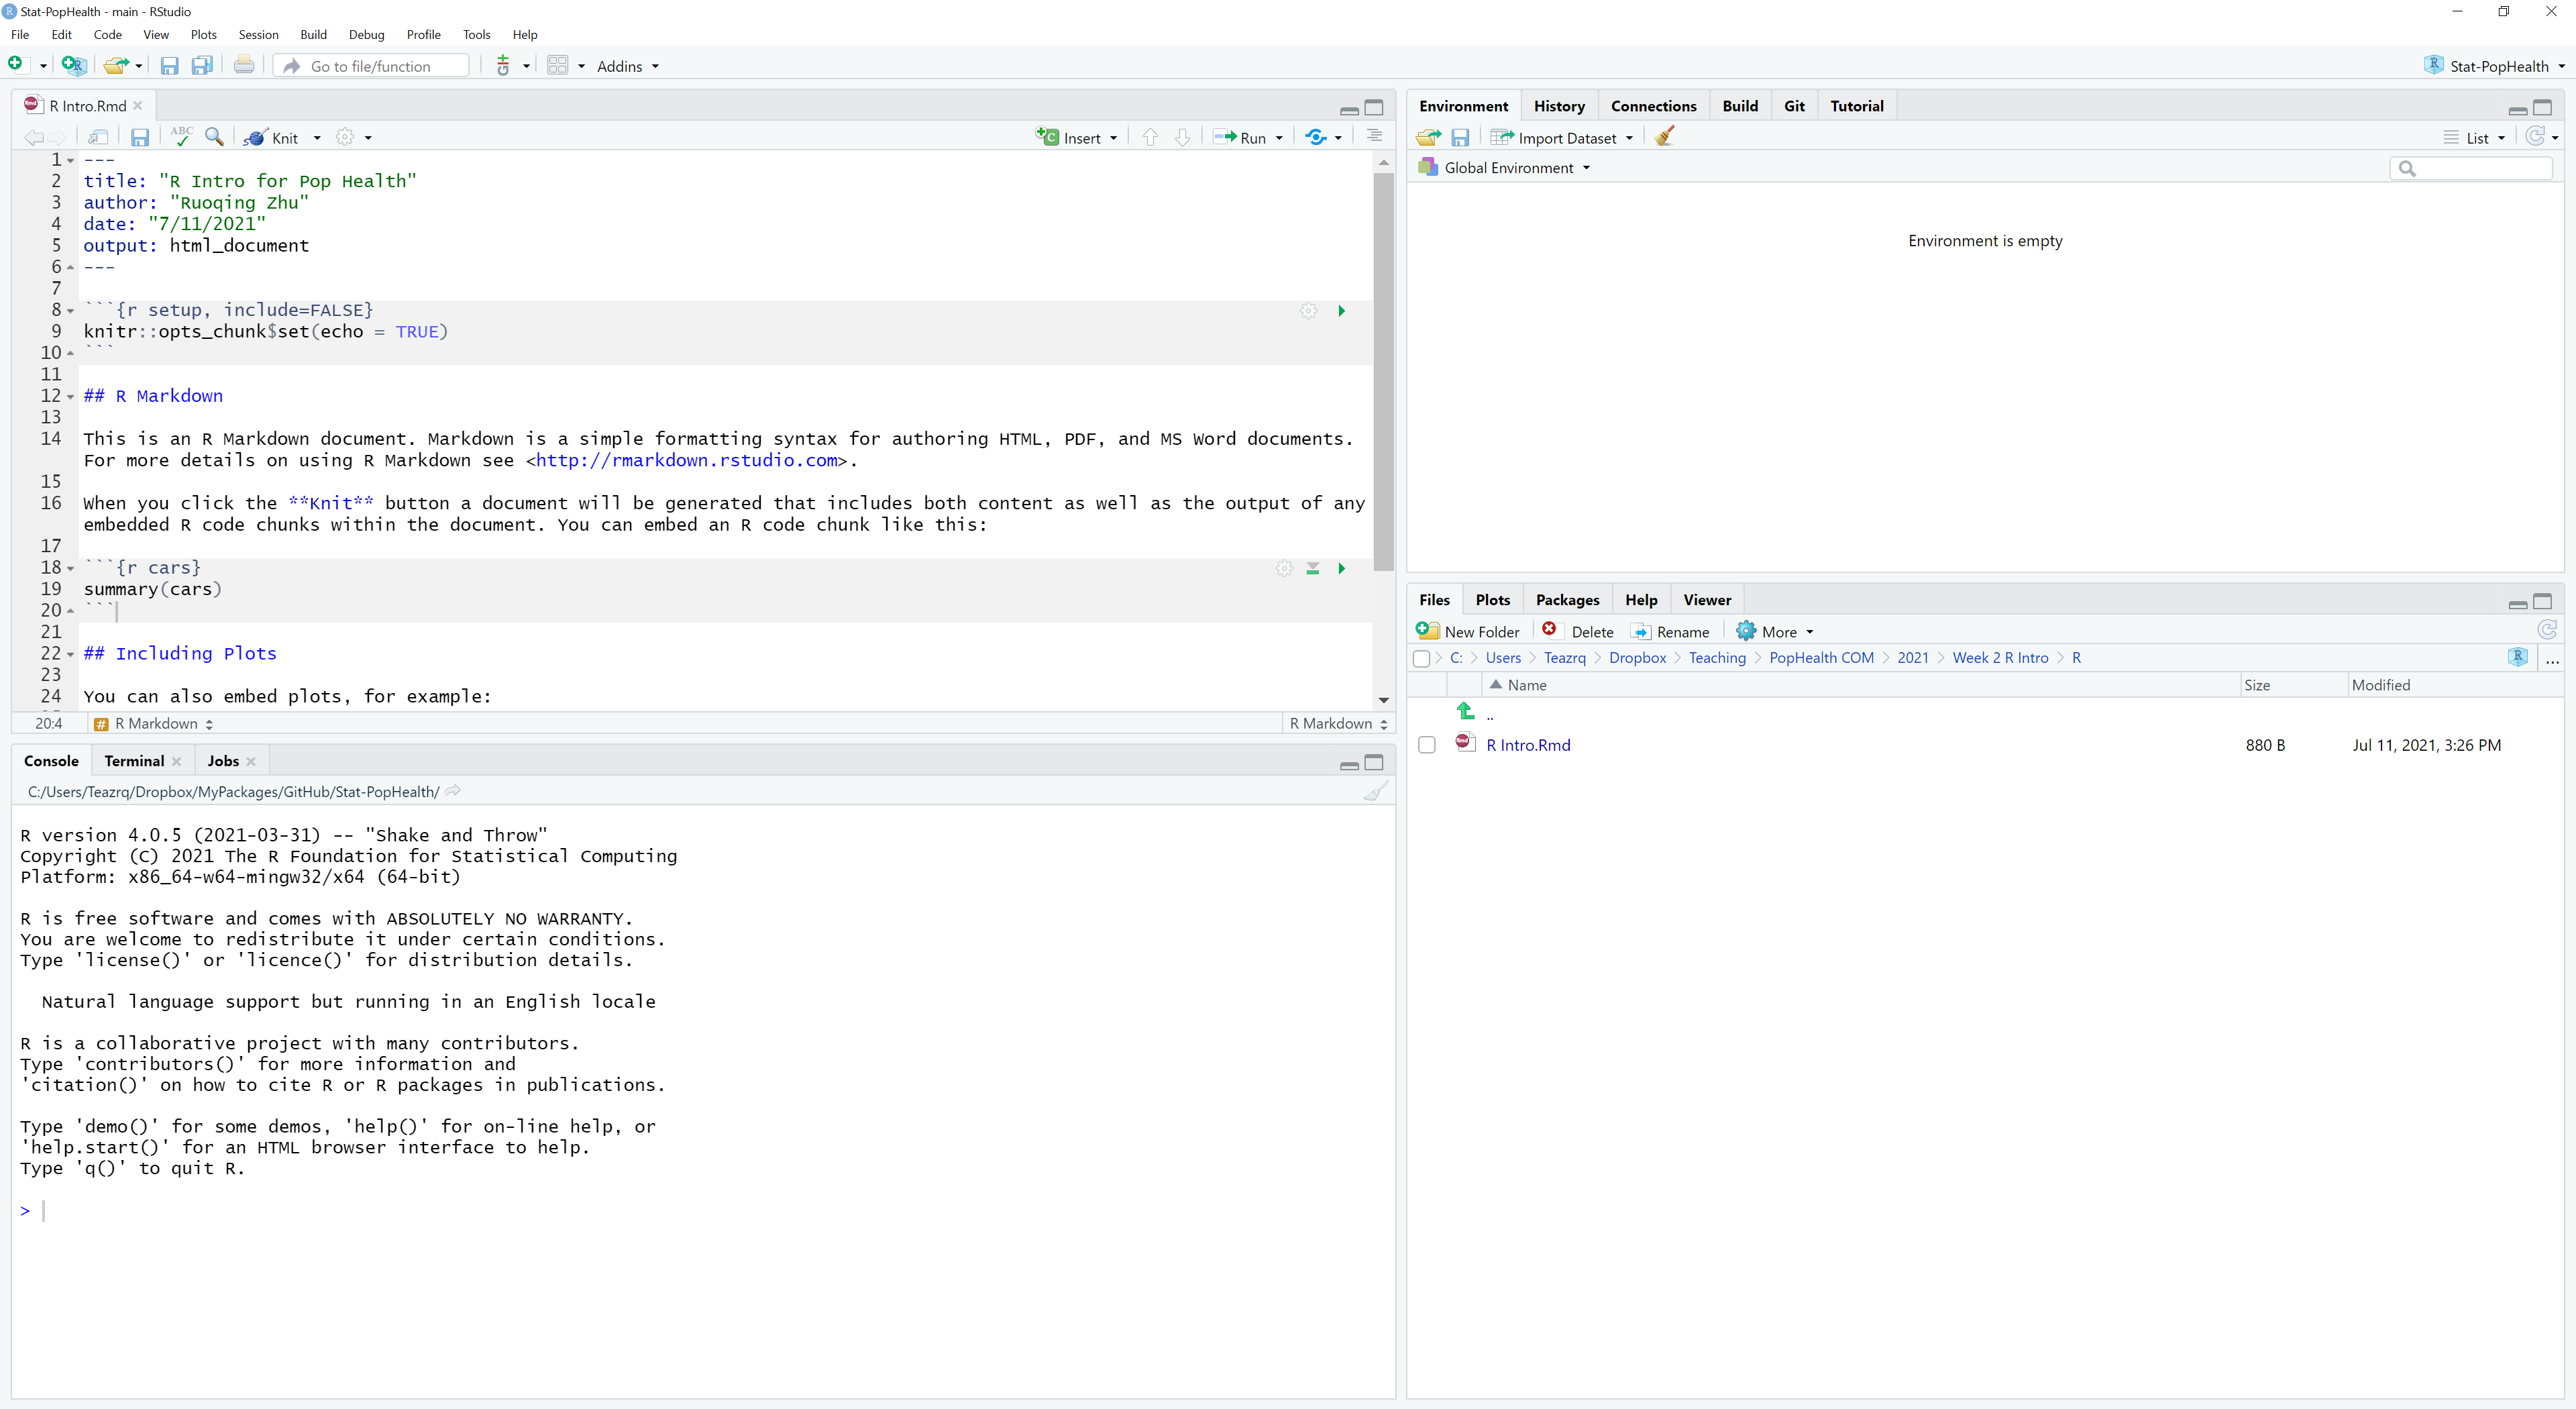
\includegraphics[width=1\textwidth,height=\textheight]{images/RStudio.png}

We will mainly use the left two panes. You can either directly input code into the console to run for results, or edit your code in a file and run them in chunks or as a whole.

\hypertarget{r-basic}{%
\section{Resources and Guides}\label{r-basic}}

There are many online resources for how to use R, RStudio. For example, David Dalpiaz's other online book \href{http://daviddalpiaz.github.io/appliedstats/}{Applied Statistics with R} contains an introduction to using them. There are also other online documentation such as

\begin{itemize}
\tightlist
\item
  \href{https://www.youtube.com/watch?v=cX532N_XLIs\&t=19s/}{Install R and RStudio}
\item
  \href{http://www.r-tutor.com/r-introduction}{R tutorial}
\item
  \href{https://www.youtube.com/playlist?list=PLBgxzZMu3GpPojVSoriMTWQCUno_3hjNi}{Data in R Play-list (video)}
\item
  \href{https://www.youtube.com/playlist?list=PLBgxzZMu3GpMjYhX7jLm5B9gEV7AOOJ5w}{R and RStudio Play-list (video)}
\end{itemize}

It is worth to mention that once you become an advanced user, and possibly a developer of R packages using \texttt{C/C++} (add-on of R for performing specific tasks), and you also happen to use Windows like I do, you will have to install \href{https://cran.r-project.org/bin/windows/Rtools/}{Rtools} that contains the gcc compilers. This is also needed if you want to install any R package from a ``source'' (\texttt{.tar.gz}) file instead of using the so-called ``binaries'' (\texttt{.zip} files).

\hypertarget{basic-mathematical-operations}{%
\section{Basic Mathematical Operations}\label{basic-mathematical-operations}}

Basic R calculations and operations should be self-explanatory. Try to type-in the following commands into your R console and start to explore yourself. Lines with a \texttt{\#} in the front are comments, which will not be executed. Lines with \texttt{\#\#} in the front are outputs you should expect.

\begin{Shaded}
\begin{Highlighting}[]
  \CommentTok{# Basic mathematical operations}
  \DecValTok{1} \OperatorTok{+}\StringTok{ }\DecValTok{3}
\CommentTok{## [1] 4}
  \DecValTok{1} \OperatorTok{-}\StringTok{ }\DecValTok{3}
\CommentTok{## [1] -2}
  \DecValTok{1} \OperatorTok{*}\StringTok{ }\DecValTok{3}
\CommentTok{## [1] 3}
  \DecValTok{1} \OperatorTok{/}\StringTok{ }\DecValTok{3}
\CommentTok{## [1] 0.3333333}
  \DecValTok{3}\OperatorTok{^}\DecValTok{5}
\CommentTok{## [1] 243}
  \DecValTok{4}\OperatorTok{^}\NormalTok{(}\OperatorTok{-}\DecValTok{1}\OperatorTok{/}\DecValTok{2}\NormalTok{)}
\CommentTok{## [1] 0.5}
\NormalTok{  pi}
\CommentTok{## [1] 3.141593}
  
  \CommentTok{# some math functions}
  \KeywordTok{sqrt}\NormalTok{(}\DecValTok{4}\NormalTok{)}
\CommentTok{## [1] 2}
  \KeywordTok{exp}\NormalTok{(}\DecValTok{1}\NormalTok{)}
\CommentTok{## [1] 2.718282}
  \KeywordTok{log}\NormalTok{(}\DecValTok{3}\NormalTok{)}
\CommentTok{## [1] 1.098612}
  \KeywordTok{log2}\NormalTok{(}\DecValTok{16}\NormalTok{)}
\CommentTok{## [1] 4}
  \KeywordTok{log}\NormalTok{(}\DecValTok{15}\NormalTok{, }\DataTypeTok{base =} \DecValTok{3}\NormalTok{)}
\CommentTok{## [1] 2.464974}
  \KeywordTok{factorial}\NormalTok{(}\DecValTok{5}\NormalTok{)}
\CommentTok{## [1] 120}
  \KeywordTok{sin}\NormalTok{(pi)}
\CommentTok{## [1] 1.224606e-16}
\end{Highlighting}
\end{Shaded}

If you want to see more information about a particular function or operator in R, the easiest way is to get the reference document. Put a question mark in front of a function name:

\begin{Shaded}
\begin{Highlighting}[]
  \CommentTok{# In a default R console window, this will open up a web browser.}
  \CommentTok{# In RStudio, this will be displayed at the ‘Help’ window at the bottom-right penal (Help tab). }
\NormalTok{  ?log10}
\NormalTok{  ?cos}
\end{Highlighting}
\end{Shaded}

\hypertarget{data-objects}{%
\section{Data Objects}\label{data-objects}}

Data objects can be a complicated topic for people who never used R before. The most common data objects are \texttt{vector}, \texttt{matrix}, \texttt{list}, and \texttt{data.frame}. They are defined using a specific syntax. To define a vector, we use \texttt{c} followed by \texttt{()}, where the elements within the parenthesis are separated using comma. You can save the vector and name as something else. For example

\begin{Shaded}
\begin{Highlighting}[]
  \CommentTok{# creating a vector}
  \KeywordTok{c}\NormalTok{(}\DecValTok{1}\NormalTok{,}\DecValTok{2}\NormalTok{,}\DecValTok{3}\NormalTok{,}\DecValTok{4}\NormalTok{)}
\end{Highlighting}
\end{Shaded}

\begin{verbatim}
## [1] 1 2 3 4
\end{verbatim}

\begin{Shaded}
\begin{Highlighting}[]
  \KeywordTok{c}\NormalTok{(}\StringTok{"a"}\NormalTok{, }\StringTok{"b"}\NormalTok{, }\StringTok{"c"}\NormalTok{)}
\end{Highlighting}
\end{Shaded}

\begin{verbatim}
## [1] "a" "b" "c"
\end{verbatim}

\begin{Shaded}
\begin{Highlighting}[]
  \CommentTok{# define a new vector object, called `x`}
\NormalTok{  x =}\StringTok{ }\KeywordTok{c}\NormalTok{(}\DecValTok{1}\NormalTok{,}\DecValTok{1}\NormalTok{,}\DecValTok{1}\NormalTok{,}\DecValTok{0}\NormalTok{,}\DecValTok{0}\NormalTok{,}\DecValTok{0}\NormalTok{)}
\end{Highlighting}
\end{Shaded}

After defining this object \texttt{x}, it should also appear on your top-right environment pane. To access elements in an object, we use the \texttt{{[}{]}} operator, like a \texttt{C} programming reference style.

\begin{Shaded}
\begin{Highlighting}[]
  \CommentTok{# getting the second element in x}
\NormalTok{  x[}\DecValTok{2}\NormalTok{]}
\end{Highlighting}
\end{Shaded}

\begin{verbatim}
## [1] 1
\end{verbatim}

\begin{Shaded}
\begin{Highlighting}[]
  \CommentTok{# getting the second to the fourth element in x}
\NormalTok{  x[}\DecValTok{2}\OperatorTok{:}\DecValTok{4}\NormalTok{]}
\end{Highlighting}
\end{Shaded}

\begin{verbatim}
## [1] 1 1 0
\end{verbatim}

Similarly, we can create and access elements in a matrix:

\begin{Shaded}
\begin{Highlighting}[]
  \CommentTok{# create a matrix by providing all of its elements}
  \CommentTok{# the elements are filled to the matrix by column}
  \KeywordTok{matrix}\NormalTok{(}\KeywordTok{c}\NormalTok{(}\DecValTok{1}\NormalTok{,}\DecValTok{2}\NormalTok{,}\DecValTok{3}\NormalTok{,}\DecValTok{4}\NormalTok{), }\DecValTok{2}\NormalTok{, }\DecValTok{2}\NormalTok{)}
\end{Highlighting}
\end{Shaded}

\begin{verbatim}
##      [,1] [,2]
## [1,]    1    3
## [2,]    2    4
\end{verbatim}

\begin{Shaded}
\begin{Highlighting}[]
  \CommentTok{# create a matrix by column-bind vectors}
\NormalTok{  y =}\StringTok{ }\KeywordTok{c}\NormalTok{(}\DecValTok{1}\NormalTok{,}\DecValTok{0}\NormalTok{,}\DecValTok{1}\NormalTok{,}\DecValTok{0}\NormalTok{,}\DecValTok{1}\NormalTok{,}\DecValTok{0}\NormalTok{)}
  \KeywordTok{cbind}\NormalTok{(x, y)}
\end{Highlighting}
\end{Shaded}

\begin{verbatim}
##      x y
## [1,] 1 1
## [2,] 1 0
## [3,] 1 1
## [4,] 0 0
## [5,] 0 1
## [6,] 0 0
\end{verbatim}

\begin{Shaded}
\begin{Highlighting}[]
  \CommentTok{# access elements in a matrix}
  \CommentTok{# Note that in R, upper and lower cases are treated as two different objects}
\NormalTok{  X =}\StringTok{ }\KeywordTok{matrix}\NormalTok{(}\KeywordTok{c}\NormalTok{(}\DecValTok{1}\OperatorTok{:}\DecValTok{16}\NormalTok{), }\DecValTok{4}\NormalTok{, }\DecValTok{4}\NormalTok{)}
\NormalTok{  X}
\end{Highlighting}
\end{Shaded}

\begin{verbatim}
##      [,1] [,2] [,3] [,4]
## [1,]    1    5    9   13
## [2,]    2    6   10   14
## [3,]    3    7   11   15
## [4,]    4    8   12   16
\end{verbatim}

\begin{Shaded}
\begin{Highlighting}[]
\NormalTok{  X[}\DecValTok{2}\NormalTok{, }\DecValTok{3}\NormalTok{]}
\end{Highlighting}
\end{Shaded}

\begin{verbatim}
## [1] 10
\end{verbatim}

\begin{Shaded}
\begin{Highlighting}[]
\NormalTok{  X[}\DecValTok{1}\NormalTok{, ]}
\end{Highlighting}
\end{Shaded}

\begin{verbatim}
## [1]  1  5  9 13
\end{verbatim}

\begin{Shaded}
\begin{Highlighting}[]
  \CommentTok{# getting a sub-matrix of X}
\NormalTok{  X[}\DecValTok{1}\OperatorTok{:}\DecValTok{2}\NormalTok{, }\DecValTok{3}\OperatorTok{:}\DecValTok{4}\NormalTok{]}
\end{Highlighting}
\end{Shaded}

\begin{verbatim}
##      [,1] [,2]
## [1,]    9   13
## [2,]   10   14
\end{verbatim}

Mathematical operations on vectors and matrices are, by default, element-wise. For matrix multiplications, you should use \texttt{\%*\%}.

\begin{Shaded}
\begin{Highlighting}[]
  \CommentTok{# adding two vectors}
\NormalTok{  (x }\OperatorTok{+}\StringTok{ }\NormalTok{y)}\OperatorTok{^}\DecValTok{2}
\end{Highlighting}
\end{Shaded}

\begin{verbatim}
## [1] 4 1 4 0 1 0
\end{verbatim}

\begin{Shaded}
\begin{Highlighting}[]
  \CommentTok{# getting the length of a vector}
  \KeywordTok{length}\NormalTok{(x)}
\end{Highlighting}
\end{Shaded}

\begin{verbatim}
## [1] 6
\end{verbatim}

\begin{Shaded}
\begin{Highlighting}[]
  \CommentTok{# matrix multiplication}
\NormalTok{  X }\OperatorTok\StringTok{ }\NormalTok{X}
\end{Highlighting}
\end{Shaded}

\begin{verbatim}
##      [,1] [,2] [,3] [,4]
## [1,]   90  202  314  426
## [2,]  100  228  356  484
## [3,]  110  254  398  542
## [4,]  120  280  440  600
\end{verbatim}

\begin{Shaded}
\begin{Highlighting}[]
  \CommentTok{# getting the dimension of a matrix}
  \KeywordTok{dim}\NormalTok{(X)}
\end{Highlighting}
\end{Shaded}

\begin{verbatim}
## [1] 4 4
\end{verbatim}

\begin{Shaded}
\begin{Highlighting}[]
  \CommentTok{# A warning will be issued when R detects something wrong}
  \CommentTok{# Results may still be produced however}
\NormalTok{  y }\OperatorTok{+}\StringTok{ }\KeywordTok{c}\NormalTok{(}\DecValTok{1}\NormalTok{,}\DecValTok{2}\NormalTok{,}\DecValTok{3}\NormalTok{,}\DecValTok{4}\NormalTok{)}
\end{Highlighting}
\end{Shaded}

\begin{verbatim}
## Warning in y + c(1, 2, 3, 4): longer object length is not a multiple of shorter object length
\end{verbatim}

\begin{verbatim}
## [1] 2 2 4 4 2 2
\end{verbatim}

\texttt{list()} creates a list of objects (of any type). However, some operators cannot be directly applied to a list in a similar way as to vectors or matrices. Model fitting results in R are usually stored as a list. For example, the \texttt{lm()} function, which will be introduced later.

\begin{Shaded}
\begin{Highlighting}[]
  \CommentTok{# creating a list}
\NormalTok{  x =}\StringTok{ }\KeywordTok{list}\NormalTok{(}\KeywordTok{c}\NormalTok{(}\DecValTok{1}\NormalTok{,}\DecValTok{2}\NormalTok{), }\StringTok{"hello"}\NormalTok{, }\KeywordTok{matrix}\NormalTok{(}\KeywordTok{c}\NormalTok{(}\DecValTok{1}\NormalTok{,}\DecValTok{2}\NormalTok{,}\DecValTok{3}\NormalTok{,}\DecValTok{4}\NormalTok{), }\DecValTok{2}\NormalTok{, }\DecValTok{2}\NormalTok{))}

  \CommentTok{# accessing its elements using double brackets `[[]]` }
\NormalTok{  x[[}\DecValTok{1}\NormalTok{]]}
\end{Highlighting}
\end{Shaded}

\begin{verbatim}
## [1] 1 2
\end{verbatim}

\texttt{data.frame()} creates a list of vectors of equal length, and display them as a matrix-like object, in which each vector is a column of the matrix. It is mainly used for storing data. This will be our most frequently used data object for analysis. For example, in the famous \texttt{iris} data, the first four columns are numerical variables, while the last column is a categorical variable with three levels: \texttt{setosa}, \texttt{versicolor}, and \texttt{virginica}:

\begin{Shaded}
\begin{Highlighting}[]
  \CommentTok{# The iris data is included with base R, so we can use them directly}
  \CommentTok{# This will create a copy of the data into your environment}
  \KeywordTok{data}\NormalTok{(iris)}

  \CommentTok{# the head function peeks the first several rows of the dataset }
  \KeywordTok{head}\NormalTok{(iris, }\DataTypeTok{n =} \DecValTok{3}\NormalTok{)}
\end{Highlighting}
\end{Shaded}

\begin{verbatim}
##   Sepal.Length Sepal.Width Petal.Length Petal.Width Species
## 1          5.1         3.5          1.4         0.2  setosa
## 2          4.9         3.0          1.4         0.2  setosa
## 3          4.7         3.2          1.3         0.2  setosa
\end{verbatim}

\begin{Shaded}
\begin{Highlighting}[]
  \CommentTok{# each column usually contains a column (variable) name }
  \KeywordTok{colnames}\NormalTok{(iris)}
\end{Highlighting}
\end{Shaded}

\begin{verbatim}
## [1] "Sepal.Length" "Sepal.Width"  "Petal.Length" "Petal.Width"  "Species"
\end{verbatim}

\begin{Shaded}
\begin{Highlighting}[]
  \CommentTok{# data frame can be called by each individual column, which will be a vector}
  \CommentTok{# iris$Species}
\NormalTok{  iris}\OperatorTok{$}\NormalTok{Species[}\DecValTok{2}\OperatorTok{:}\DecValTok{4}\NormalTok{]}
\end{Highlighting}
\end{Shaded}

\begin{verbatim}
## [1] setosa setosa setosa
## Levels: setosa versicolor virginica
\end{verbatim}

\begin{Shaded}
\begin{Highlighting}[]
  \CommentTok{# the summary function can be used to view summary statistics of all variables}
  \KeywordTok{summary}\NormalTok{(iris)}
\end{Highlighting}
\end{Shaded}

\begin{verbatim}
##   Sepal.Length    Sepal.Width     Petal.Length    Petal.Width          Species  
##  Min.   :4.300   Min.   :2.000   Min.   :1.000   Min.   :0.100   setosa    :50  
##  1st Qu.:5.100   1st Qu.:2.800   1st Qu.:1.600   1st Qu.:0.300   versicolor:50  
##  Median :5.800   Median :3.000   Median :4.350   Median :1.300   virginica :50  
##  Mean   :5.843   Mean   :3.057   Mean   :3.758   Mean   :1.199                  
##  3rd Qu.:6.400   3rd Qu.:3.300   3rd Qu.:5.100   3rd Qu.:1.800                  
##  Max.   :7.900   Max.   :4.400   Max.   :6.900   Max.   :2.500
\end{verbatim}

\texttt{factor} is a special type of vector. It is frequently used to store a categorical variable with more than two categories. The last column of the iris data is a factor. You need to be a little bit careful when dealing with factor variables when during modeling since some functions do not take care of them automatically or they do it in a different way than you thought. For example, changing a factor variable into numerical ones will ignore any potential relationship among different categories.

\begin{Shaded}
\begin{Highlighting}[]
  \KeywordTok{levels}\NormalTok{(iris}\OperatorTok{$}\NormalTok{Species)}
\end{Highlighting}
\end{Shaded}

\begin{verbatim}
## [1] "setosa"     "versicolor" "virginica"
\end{verbatim}

\begin{Shaded}
\begin{Highlighting}[]
  \KeywordTok{as.numeric}\NormalTok{(iris}\OperatorTok{$}\NormalTok{Species)}
\end{Highlighting}
\end{Shaded}

\begin{verbatim}
##   [1] 1 1 1 1 1 1 1 1 1 1 1 1 1 1 1 1 1 1 1 1 1 1 1 1 1 1 1 1 1 1 1 1 1 1 1 1 1 1 1 1 1 1 1 1 1 1 1 1 1 1 2 2 2 2 2 2 2 2 2 2 2 2 2 2 2 2 2 2 2 2 2 2 2 2 2 2 2 2 2 2 2 2 2 2 2 2 2 2 2 2 2 2 2 2 2 2 2 2 2 2 3 3 3 3 3 3 3 3 3 3 3 3 3 3 3 3 3 3 3 3 3 3 3 3 3 3 3 3 3 3 3 3 3 3 3 3 3 3 3 3 3 3 3 3 3 3 3 3 3 3
\end{verbatim}

\hypertarget{readin-and-save-data}{%
\section{Readin and save data}\label{readin-and-save-data}}

Data can be imported from a variety of sources. More commonly, a dataset can be stored in \texttt{.txt} and \texttt{.csv} files. Such data reading methods require specific structures in the source file: the first row should contain column names, and there should be equal number of elements in each row. Hence you should always check your file before reading them in.

\begin{Shaded}
\begin{Highlighting}[]
  \CommentTok{# read-in data}
\NormalTok{  birthrate =}\StringTok{ }\KeywordTok{read.csv}\NormalTok{(}\StringTok{"data/birthrate.csv"}\NormalTok{)}
  \KeywordTok{head}\NormalTok{(birthrate)}
\end{Highlighting}
\end{Shaded}

\begin{verbatim}
##   Year Birthrate
## 1 1917     183.1
## 2 1918     183.9
## 3 1919     163.1
## 4 1920     179.5
## 5 1921     181.4
## 6 1922     173.4
\end{verbatim}

\begin{Shaded}
\begin{Highlighting}[]
  \CommentTok{# to see how many observations (rows) and variables (columns) in a dataset}
  \KeywordTok{dim}\NormalTok{(birthrate)}
\end{Highlighting}
\end{Shaded}

\begin{verbatim}
## [1] 87  2
\end{verbatim}

R data can also be saved into other formats. The more efficient way, assuming that you are going to load these file back to R in the future, is to save them as \texttt{.RData} file. Usually, for a larger dataset, this reduces the time spend on reading the data.

\begin{Shaded}
\begin{Highlighting}[]
  \CommentTok{# saving a object to .RData file}
  \KeywordTok{save}\NormalTok{(birthrate, }\DataTypeTok{file =} \StringTok{"mydata.RData"}\NormalTok{)}

  \CommentTok{# you can specify multiple objects to be saved into the same file}
  \KeywordTok{save}\NormalTok{(birthrate, iris, }\DataTypeTok{file =} \StringTok{"mydata.RData"}\NormalTok{)}
  
  \CommentTok{# load the data again back to your environment}
  \KeywordTok{load}\NormalTok{(}\StringTok{"mydata.RData"}\NormalTok{)}
  
  \CommentTok{# alternatively, you can also save data to a .csv file}
  \KeywordTok{write.csv}\NormalTok{(birthrate, }\DataTypeTok{file =} \StringTok{"mydata.csv"}\NormalTok{)}
  
  \CommentTok{# you can notice that this .csv file contains an extra column of "ID number", without a column name}
  \CommentTok{# Hence, when you read this file back into R, you should specify `row.names = 1` to indicate that.}
  \CommentTok{# Otherwise this will produce an error}
  \KeywordTok{read.csv}\NormalTok{(}\DataTypeTok{file =} \StringTok{"mydata.csv"}\NormalTok{, }\DataTypeTok{row.names =} \DecValTok{1}\NormalTok{)}
\end{Highlighting}
\end{Shaded}

\hypertarget{using-and-defining-functions}{%
\section{Using and defining functions}\label{using-and-defining-functions}}

We have already used many functions. You can also define your own functions, and even build them into packages (more on this later) for other people to use. This is the main advantage of R. For example, let's consider writing a function that returns the minimum and maximum of a vector. Suppose we already know the \texttt{min()} and \texttt{max()} functions.

\begin{Shaded}
\begin{Highlighting}[]
\NormalTok{  myrange <-}\StringTok{ }\ControlFlowTok{function}\NormalTok{(x) }\CommentTok{# x is the argument that your function takes in}
\NormalTok{  \{}
    \KeywordTok{return}\NormalTok{(}\KeywordTok{c}\NormalTok{(}\KeywordTok{min}\NormalTok{(x), }\KeywordTok{max}\NormalTok{(x))) }\CommentTok{# return a vector that contains two elements}
\NormalTok{  \}}

\NormalTok{  x =}\StringTok{ }\DecValTok{1}\OperatorTok{:}\DecValTok{10}
  \KeywordTok{myrange}\NormalTok{(x)}
\end{Highlighting}
\end{Shaded}

\begin{verbatim}
## [1]  1 10
\end{verbatim}

\begin{Shaded}
\begin{Highlighting}[]
  \CommentTok{# R already has this function}
  \KeywordTok{range}\NormalTok{(x)}
\end{Highlighting}
\end{Shaded}

\begin{verbatim}
## [1]  1 10
\end{verbatim}

\hypertarget{distribution-and-random-numbers}{%
\section{Distribution and random numbers}\label{distribution-and-random-numbers}}

Three distributions that are most frequently used in this course are Bernoulli, Gaussian (normal), and \(t\) distributions. Bernoulli distributions can be used to describe binary variables, while Gaussian distribution is often used to describe continuous ones. The following code generates some random variables

\begin{Shaded}
\begin{Highlighting}[]
  \CommentTok{# read the documentation of rbinom() using ?rbinom}
\NormalTok{  x =}\StringTok{ }\KeywordTok{rbinom}\NormalTok{(}\DecValTok{100}\NormalTok{, }\DecValTok{1}\NormalTok{, }\FloatTok{0.4}\NormalTok{)}
  \KeywordTok{table}\NormalTok{(x)}
\end{Highlighting}
\end{Shaded}

\begin{verbatim}
## x
##  0  1 
## 62 38
\end{verbatim}

However, this result cannot be replicated by others, since the next time we run this code, the random numbers will be different. Hence it is important to set and keep the random seed when a random algorithm is involved. The following code will always generate the same result

\begin{Shaded}
\begin{Highlighting}[]
  \KeywordTok{set.seed}\NormalTok{(}\DecValTok{1}\NormalTok{)}
\NormalTok{  x =}\StringTok{ }\KeywordTok{rbinom}\NormalTok{(}\DecValTok{100}\NormalTok{, }\DecValTok{1}\NormalTok{, }\FloatTok{0.4}\NormalTok{)}
\NormalTok{  y =}\StringTok{ }\KeywordTok{rnorm}\NormalTok{(}\DecValTok{100}\NormalTok{) }\CommentTok{# by default, this is mean 0 and variance 1}
  
  \KeywordTok{table}\NormalTok{(x)}
\end{Highlighting}
\end{Shaded}

\begin{verbatim}
## x
##  0  1 
## 57 43
\end{verbatim}

\begin{Shaded}
\begin{Highlighting}[]
  \KeywordTok{hist}\NormalTok{(y)}
\end{Highlighting}
\end{Shaded}

\begin{center}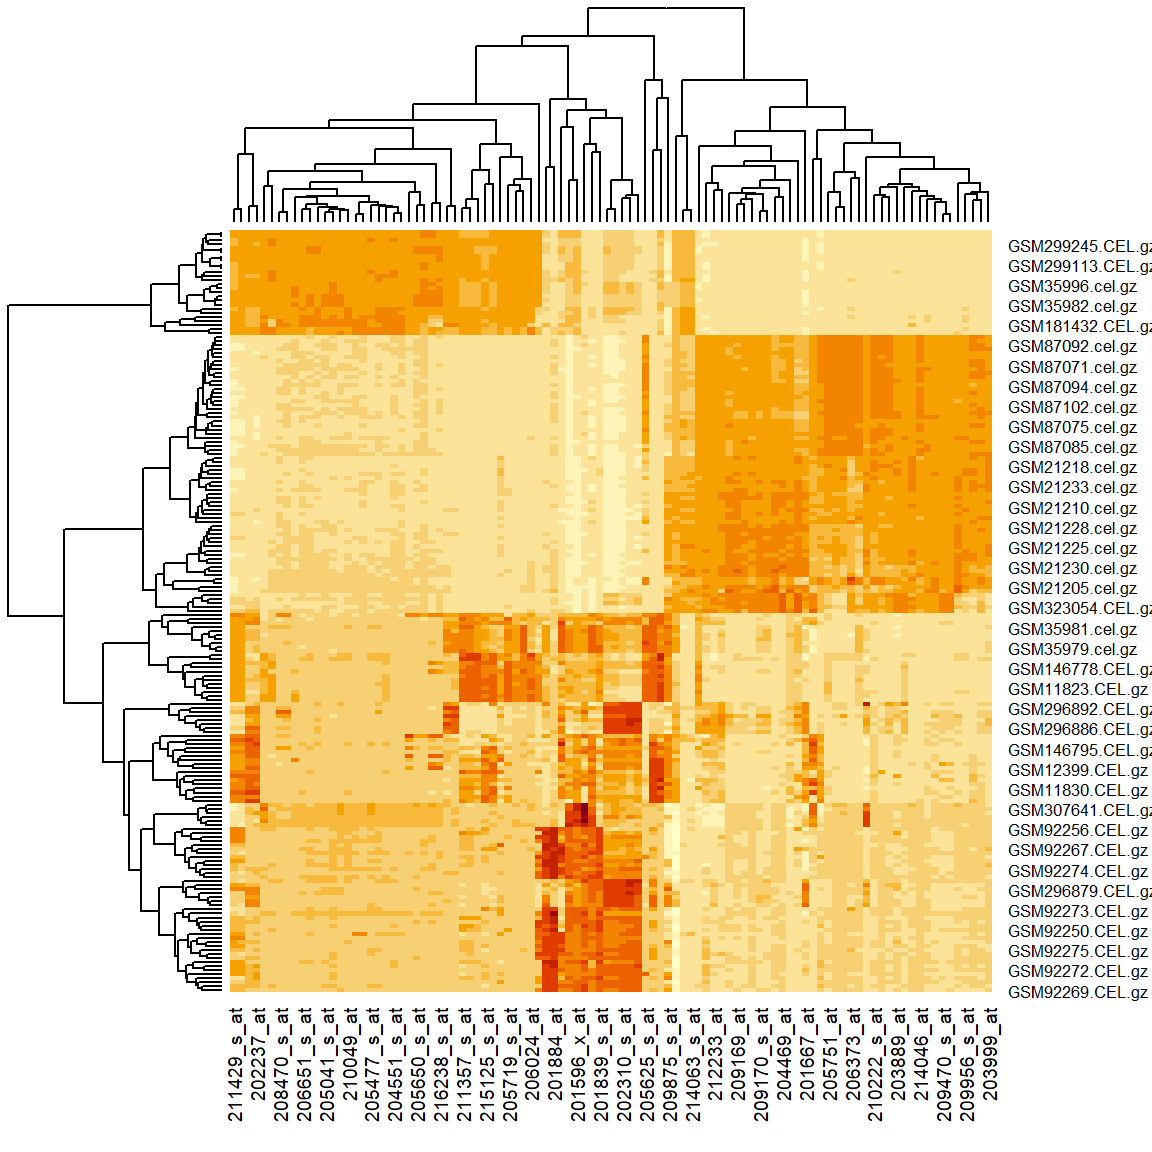
\includegraphics[width=0.6\linewidth]{SMLR_files/figure-latex/unnamed-chunk-15-1} \end{center}

\begin{Shaded}
\begin{Highlighting}[]
  \KeywordTok{boxplot}\NormalTok{(y }\OperatorTok{~}\StringTok{ }\NormalTok{x)}
\end{Highlighting}
\end{Shaded}

\begin{center}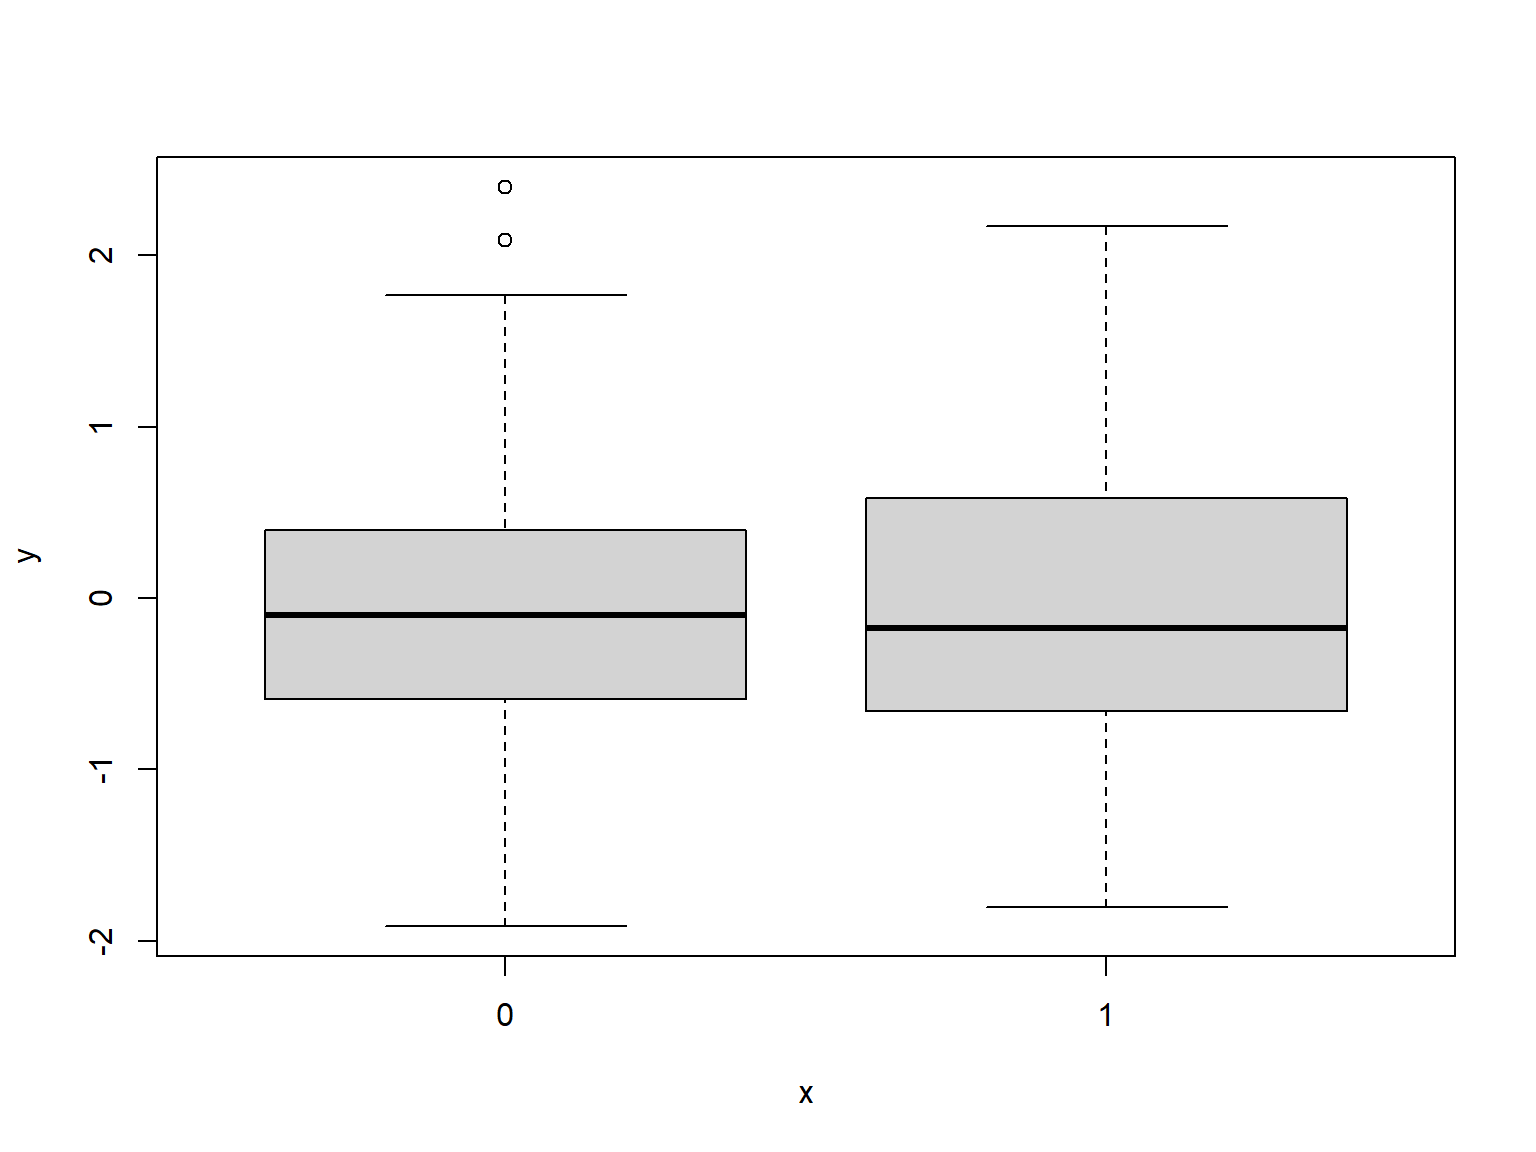
\includegraphics[width=0.6\linewidth]{SMLR_files/figure-latex/unnamed-chunk-15-2} \end{center}

\hypertarget{using-packages-and-other-resources}{%
\section{Using packages and other resources}\label{using-packages-and-other-resources}}

Packages are written and contributed to R by individuals. They provide additional features (functions or data) that serve particular needs. For example, the \texttt{ggplot2} package is developed by the RStudio team that provides nice features to plot data. We will have more examples of this later on, but first, let's install and load the package so that we can use these features. More details will be provided in the data visualization section.

\begin{Shaded}
\begin{Highlighting}[]
  \CommentTok{# to install a package}
  \KeywordTok{install.packages}\NormalTok{(}\StringTok{"ggplot2"}\NormalTok{)}
\end{Highlighting}
\end{Shaded}

\begin{Shaded}
\begin{Highlighting}[]
  \CommentTok{# to load the package}
  \KeywordTok{library}\NormalTok{(ggplot2)}

  \CommentTok{# use the ggplot() function to produce a plot}
  \CommentTok{# Sepal.Length is the horizontal axis}
  \CommentTok{# Sepal.Width is the vertical axis}
  \CommentTok{# Species labels are used as color}
  \KeywordTok{ggplot}\NormalTok{(iris, }\KeywordTok{aes}\NormalTok{(Sepal.Length, Sepal.Width, }\DataTypeTok{colour =}\NormalTok{ Species)) }\OperatorTok{+}\StringTok{ }
\StringTok{    }\KeywordTok{geom_point}\NormalTok{()  }
\end{Highlighting}
\end{Shaded}

\begin{center}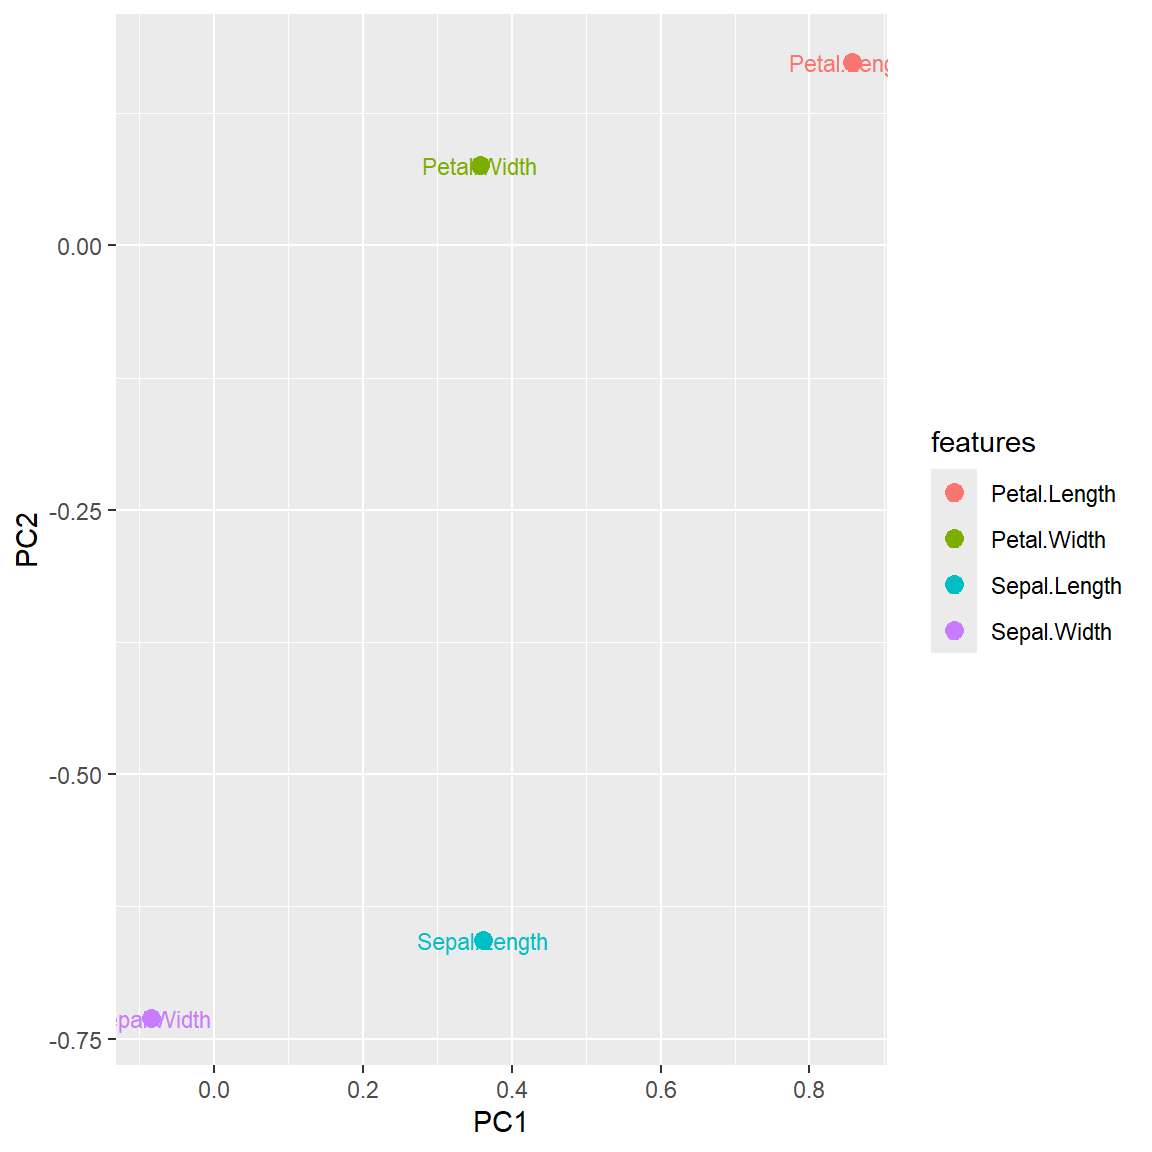
\includegraphics[width=0.6\linewidth]{SMLR_files/figure-latex/unnamed-chunk-17-1} \end{center}

You may also noticed that in our previous examples, all tables only displayed the first several rows. One may be interested in looking at the entire dataset, however, it would take too much space to display the whole table. Here is a package that would allow you to display it in a compact window. It also provides searching and sorting tools. You can integrate this into your R Markdown reports.

\begin{Shaded}
\begin{Highlighting}[]
  \KeywordTok{library}\NormalTok{(DT)}
  \KeywordTok{datatable}\NormalTok{(iris, }\DataTypeTok{filter =} \StringTok{"top"}\NormalTok{, }\DataTypeTok{rownames =} \OtherTok{FALSE}\NormalTok{,}
            \DataTypeTok{options =} \KeywordTok{list}\NormalTok{(}\DataTypeTok{pageLength =} \DecValTok{5}\NormalTok{))}
\end{Highlighting}
\end{Shaded}

Often times, you may want to perform a new task and you don't know what function can be used to achieve that. Google Search or Stack Overflow are probably your best friends. I used to encounter this problem: I have a list of objects, and each of them is a vector. I then need to extract the first element of all these vectors. However, doing this using a for-loop can be slow, and I am also interested in a cleaner code. So I found \href{https://stackoverflow.com/questions/44176908/r-list-get-first-item-of-each-element}{this post}, which provided a simple answer:

\begin{Shaded}
\begin{Highlighting}[]
  \CommentTok{# create the list}
\NormalTok{  a =}\StringTok{ }\KeywordTok{list}\NormalTok{(}\KeywordTok{c}\NormalTok{(}\DecValTok{1}\NormalTok{,}\DecValTok{1}\NormalTok{,}\DecValTok{1}\NormalTok{), }\KeywordTok{c}\NormalTok{(}\DecValTok{2}\NormalTok{,}\DecValTok{2}\NormalTok{,}\DecValTok{2}\NormalTok{), }\KeywordTok{c}\NormalTok{(}\DecValTok{3}\NormalTok{,}\DecValTok{3}\NormalTok{,}\DecValTok{3}\NormalTok{))}
  
  \CommentTok{# extract the first element in each vector of the list}
  \KeywordTok{sapply}\NormalTok{(a, }\StringTok{"[["}\NormalTok{, }\DecValTok{1}\NormalTok{)}
\end{Highlighting}
\end{Shaded}

\begin{verbatim}
## [1] 1 2 3
\end{verbatim}

\hypertarget{practice-questions}{%
\section{Practice questions}\label{practice-questions}}

\begin{enumerate}
\def\labelenumi{\arabic{enumi}.}
\tightlist
\item
  Attach a new numerical column to the \texttt{iris} data, as the product of \texttt{Petal.Length} and \texttt{Petal.Width} and name the column as \texttt{Petal.Prod}.
\end{enumerate}

\begin{Shaded}
\begin{Highlighting}[]
\NormalTok{  iris =}\StringTok{ }\KeywordTok{cbind}\NormalTok{(iris, }\StringTok{"Petal.Prod"}\NormalTok{ =}\StringTok{ }\NormalTok{iris}\OperatorTok{$}\NormalTok{Petal.Length}\OperatorTok{*}\NormalTok{iris}\OperatorTok{$}\NormalTok{Petal.Width)}
  \KeywordTok{head}\NormalTok{(iris)}
\end{Highlighting}
\end{Shaded}

\begin{enumerate}
\def\labelenumi{\arabic{enumi}.}
\setcounter{enumi}{1}
\tightlist
\item
  Attach a new numerical column to the \texttt{iris} data, with value 1 if the observation is \texttt{setosa}, 2 for \texttt{versicolor} and 3 for \texttt{virginica}, and name the column as \texttt{Species.Num}.
\end{enumerate}

\begin{Shaded}
\begin{Highlighting}[]
\NormalTok{  iris =}\StringTok{ }\KeywordTok{cbind}\NormalTok{(iris, }\StringTok{"Species.Num"}\NormalTok{ =}\StringTok{ }\KeywordTok{as.numeric}\NormalTok{(iris}\OperatorTok{$}\NormalTok{Species))}
  \KeywordTok{head}\NormalTok{(iris)}
\end{Highlighting}
\end{Shaded}

\begin{enumerate}
\def\labelenumi{\arabic{enumi}.}
\setcounter{enumi}{2}
\tightlist
\item
  Change \texttt{Species.Num} to a factor variable such that it takes value ``Type1'' if the observation is \texttt{setosa} and ``NA'' otherwise.
\end{enumerate}

\begin{Shaded}
\begin{Highlighting}[]
\NormalTok{  iris}\OperatorTok{$}\NormalTok{Species.Num =}\StringTok{ }\KeywordTok{as.factor}\NormalTok{(}\KeywordTok{ifelse}\NormalTok{(iris}\OperatorTok{$}\NormalTok{Species }\OperatorTok{==}\StringTok{ "setosa"}\NormalTok{, }\StringTok{"Type1"}\NormalTok{, }\StringTok{"NA"}\NormalTok{))}
  \KeywordTok{head}\NormalTok{(iris)}
\end{Highlighting}
\end{Shaded}

\begin{enumerate}
\def\labelenumi{\arabic{enumi}.}
\setcounter{enumi}{3}
\tightlist
\item
  Define a function that takes in a numerical vector, and output the mean of that vector. Do this without using the \texttt{mean()} and \texttt{sum()} function.
\end{enumerate}

\begin{Shaded}
\begin{Highlighting}[]
\NormalTok{  mymean <-}\StringTok{ }\ControlFlowTok{function}\NormalTok{(x)}
\NormalTok{  \{}
\NormalTok{    sum =}\StringTok{ }\DecValTok{0}
    \ControlFlowTok{for}\NormalTok{ (i }\ControlFlowTok{in} \DecValTok{1}\OperatorTok{:}\KeywordTok{length}\NormalTok{(x))}
\NormalTok{      sum =}\StringTok{ }\NormalTok{sum }\OperatorTok{+}\StringTok{ }\NormalTok{x[i]}
    
    \KeywordTok{return}\NormalTok{(}\DataTypeTok{sum =}\NormalTok{ sum }\OperatorTok{/}\StringTok{ }\KeywordTok{length}\NormalTok{(x))}
\NormalTok{  \}}
  
\NormalTok{  x =}\StringTok{ }\DecValTok{1}\OperatorTok{:}\DecValTok{10}
  \KeywordTok{mymean}\NormalTok{(x)}
  
  \KeywordTok{mean}\NormalTok{(x)}
\end{Highlighting}
\end{Shaded}

\hypertarget{rmarkdown}{%
\chapter{RMarkdown}\label{rmarkdown}}

\hypertarget{basics-and-resources}{%
\section{Basics and Resources}\label{basics-and-resources}}

R Markdown is a built-in feature of RStudio. It integrates plain text with chunks of R code in to a single file, which is extremely useful when constructing class notes or building a website. A \texttt{.rmd} file can be compiled into nice-looking \texttt{.html}, \texttt{.pdf}, and \texttt{.docx} file. For example, this entire guide is created using R Markdown. With RStudio, you can install R Markdown from R console using the following code. Note that this should be automatically done the first time you create and compile a \texttt{.rmd} file in RStudio.

\begin{Shaded}
\begin{Highlighting}[]
  \CommentTok{# Install R Markdown from CRAN}
  \KeywordTok{install.packages}\NormalTok{(}\StringTok{"rmarkdown"}\NormalTok{)}
\end{Highlighting}
\end{Shaded}

Again there are many online guides for R Markdown, and these may not be the best ones.

\begin{itemize}
\tightlist
\item
  \href{https://bookdown.org/yihui/rmarkdown/}{R Markdown: The Definitive Guide}
\item
  \href{https://www.rstudio.com/wp-content/uploads/2015/02/rmarkdown-cheatsheet.pdf}{R Markdown Cheat Sheet}
\item
  \href{https://www.youtube.com/playlist?list=PLBgxzZMu3GpNgd07DwmS-2odHtMO6MWGH}{R Markdown Play-list (video)}
\end{itemize}

To get started, create an R Markdown template file by clicking \texttt{File} -\textgreater{} \texttt{New\ File} -\textgreater{} \texttt{R\ Markdown...}

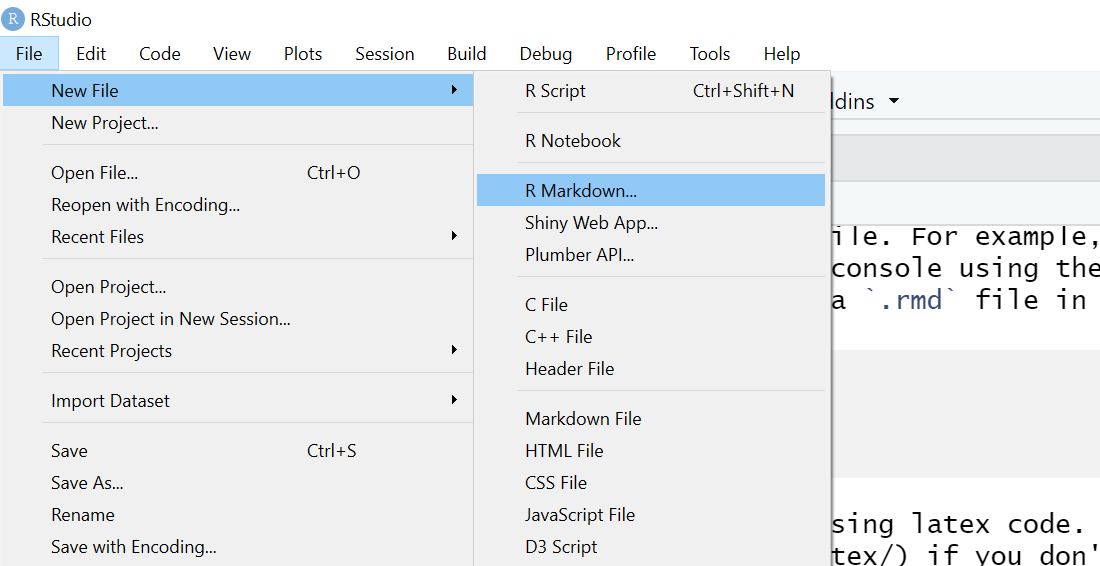
\includegraphics[width=0.7\textwidth,height=\textheight]{images/Create.png}

You can then \texttt{Knit} the template file and start to explore its features.

\includegraphics[width=0.7\textwidth,height=\textheight]{images/Knit.png}

Please note that this guide is provided in the \texttt{.html} format. However, your homework report should be in \texttt{.pdf} format. This can be done by selecting the \texttt{Knit\ to\ PDF} option from the Knit button. Again there are many online guides, and these may not be the best ones.

\begin{itemize}
\tightlist
\item
  \href{https://www.rstudio.com/wp-content/uploads/2015/02/rmarkdown-cheatsheet.pdf}{R Markdown Cheat Sheet}
\item
  \href{https://www.youtube.com/playlist?list=PLBgxzZMu3GpNgd07DwmS-2odHtMO6MWGH}{R Markdown Play-list (video)}
\end{itemize}

\hypertarget{formatting-text}{%
\section{Formatting Text}\label{formatting-text}}

Formatting text is easy. Bold can be done using \texttt{**} or \texttt{\_\_} before and after the text. Italics can be done using \texttt{*} or \texttt{\_} before and after the text. For example, \textbf{This is bold.} \emph{This is italics.} and \textbf{\emph{this is bold italics}}. \texttt{This\ text\ appears\ as\ monospaced.}

\begin{itemize}
\tightlist
\item
  Unordered list element 1.
\item
  Unordered list element 2.
\item
  Unordered list element 3.
\end{itemize}

\begin{enumerate}
\def\labelenumi{\arabic{enumi}.}
\tightlist
\item
  Ordered list element 1.
\item
  Ordered list element 2.
\item
  Ordered list element 3.
\end{enumerate}

We could mix lists and links. Note that a link can be constructed in the format \texttt{{[}display\ text{]}(http\ link)}. If colors are desired, we can customize it using, for example, \texttt{{[}\textbackslash{}textcolor\{blue\}\{display\ text\}{]}(http\ link)}. But this only works in \texttt{.pdf} format. For \texttt{.html}, use \texttt{\textless{}span\ style="color:\ red;"\textgreater{}text\textless{}/span\textgreater{}}.

\begin{itemize}
\tightlist
\item
  A default link: \href{http://rmarkdown.rstudio.com/}{RMarkdown Documentation}
\item
  colored link 1: \href{https://www.rstudio.com/wp-content/uploads/2015/02/rmarkdown-cheatsheet.pdf}{\textcolor{blue}{RMarkdown Cheatsheet}} (Not shown because it only works in PDF)
\item
  colored link 2: \href{http://www.tablesgenerator.com/markdown_tables}{{Table Generator}} (only works in HTML)
\end{itemize}

Tables are sometimes tricky using Markdown. See the above link for a helpful Markdown table generator. Note that you can also adjust the alignment by using a \texttt{:} sign.

\begin{longtable}[]{@{}cll@{}}
\toprule
A & B & C\tabularnewline
\midrule
\endhead
1 & 2 & 3\tabularnewline
Middle & Left & Right\tabularnewline
\bottomrule
\end{longtable}

\hypertarget{adding-r-code}{%
\section{\texorpdfstring{Adding \texttt{R} Code}{Adding R Code}}\label{adding-r-code}}

So far we have only used Markdown to create the text part. This is useful by itself, but the real power of RMarkdown comes when we add \texttt{R}. There are two ways we can do this. We can use \texttt{R} code chunks, or run \texttt{R} inline.

\hypertarget{r-chunks}{%
\subsection{\texorpdfstring{\texttt{R} Chunks}{R Chunks}}\label{r-chunks}}

The following is an example of an \texttt{R} code chunk

\texttt{\textasciigrave{}\textasciigrave{}\textasciigrave{}\{r\}}

\(\quad\) \texttt{set.seed(123)}

\(\quad\) \texttt{rnorm(5)}

\texttt{\textasciigrave{}\textasciigrave{}\textasciigrave{}}

This generates five random observations from the standard normal distribution. We also set the seed so that the results can be later on replicated. The result looks like the following

\begin{Shaded}
\begin{Highlighting}[]
  \KeywordTok{set.seed}\NormalTok{(}\DecValTok{123}\NormalTok{)}
  \KeywordTok{rnorm}\NormalTok{(}\DecValTok{5}\NormalTok{)}
\end{Highlighting}
\end{Shaded}

\begin{verbatim}
## [1] -0.56047565 -0.23017749  1.55870831  0.07050839  0.12928774
\end{verbatim}

\begin{Shaded}
\begin{Highlighting}[]
  \CommentTok{# define function}
\NormalTok{  get_sd =}\StringTok{ }\ControlFlowTok{function}\NormalTok{(x, }\DataTypeTok{biased =} \OtherTok{FALSE}\NormalTok{) \{}
\NormalTok{    n =}\StringTok{ }\KeywordTok{length}\NormalTok{(x) }\OperatorTok{-}\StringTok{ }\DecValTok{1} \OperatorTok{*}\StringTok{ }\OperatorTok{!}\NormalTok{biased}
    \KeywordTok{sqrt}\NormalTok{((}\DecValTok{1} \OperatorTok{/}\StringTok{ }\NormalTok{n) }\OperatorTok{*}\StringTok{ }\KeywordTok{sum}\NormalTok{((x }\OperatorTok{-}\StringTok{ }\KeywordTok{mean}\NormalTok{(x)) }\OperatorTok{^}\StringTok{ }\DecValTok{2}\NormalTok{))}
\NormalTok{  \}}
  
  \CommentTok{# generate random sample data}
  \KeywordTok{set.seed}\NormalTok{(}\DecValTok{42}\NormalTok{)}
\NormalTok{  (}\DataTypeTok{test_sample =} \KeywordTok{rnorm}\NormalTok{(}\DataTypeTok{n =} \DecValTok{10}\NormalTok{, }\DataTypeTok{mean =} \DecValTok{2}\NormalTok{, }\DataTypeTok{sd =} \DecValTok{5}\NormalTok{))}
\end{Highlighting}
\end{Shaded}

\begin{verbatim}
##  [1]  8.8547922 -0.8234909  3.8156421  5.1643130  4.0213416  1.4693774  9.5576100  1.5267048 12.0921186  1.6864295
\end{verbatim}

\begin{Shaded}
\begin{Highlighting}[]
  \CommentTok{# run function on generated data}
  \KeywordTok{get_sd}\NormalTok{(test_sample)}
\end{Highlighting}
\end{Shaded}

\begin{verbatim}
## [1] 4.177244
\end{verbatim}

There is a lot going on here. In the \texttt{.Rmd} file, notice the syntax that creates and ends the chunk. Also note that \texttt{example\_chunk} is the chunk name. Everything between the start and end syntax must be valid \texttt{R} code. Chunk names are not necessary, but can become useful as your documents grow in size.

In this example, we define a function, generate some random data in a reproducible manner, displayed the data, then ran our function.

\hypertarget{inline-r}{%
\subsection{\texorpdfstring{Inline \texttt{R}}{Inline R}}\label{inline-r}}

\texttt{R} can also be run in the middle of the exposition. For example, the mean of the data we generated is 4.7364838.

\hypertarget{importing-data}{%
\section{Importing Data}\label{importing-data}}

When using RMarkdown, any time you \emph{knit} your document to its final form, say \texttt{.html}, a number of programs run in the background. Your current \texttt{R} environment seen in RStudio will be reset. Any objects you created while working interactively inside RStudio will be ignored. Essentially a new \texttt{R} session will be spawned in the background and the code in your document is run there from start to finish. For this reason, things such as importing data must be explicitly coded into your document.

\begin{Shaded}
\begin{Highlighting}[]
  \KeywordTok{library}\NormalTok{(readr)}
\NormalTok{  example_data =}\StringTok{ }\KeywordTok{read_table}\NormalTok{(}\StringTok{"data/skincancer.txt"}\NormalTok{)}
\end{Highlighting}
\end{Shaded}

The above loads the online file. In many cases, you will load a file that is locally stored in your own computer. In that case, you can either specify the full file path, or simply use, for example \texttt{read\_csv("filename.csv")} if that file is stored at your \textbf{working directory}. The \textbf{working directory} will usually be the directory that contains your \texttt{.Rmd} file. You are recommended to reference data in this manner. Note that we use the newer \texttt{read\_csv()} from the \texttt{readr} package instead of the default \texttt{read.csv()}.

\hypertarget{working-directory}{%
\section{Working Directory}\label{working-directory}}

Whenever \texttt{R} code is run, there is always a current working directory. This allows for relative references to external files, in addition to absolute references. Since the working directory when knitting a file is always the directory that contains the \texttt{.Rmd} file, it can be helpful to set the working directory inside RStudio to match while working interactively.

To do so, select \texttt{Session\ \textgreater{}\ Set\ Working\ Directory\ \textgreater{}\ To\ Source\ File\ Location} while editing a \texttt{.Rmd} file. This will set the working directory to the path that contains the \texttt{.Rmd}. You can also use \texttt{getwd()} and \texttt{setwd()} to manipulate your working directory programmatically. These should only be used interactively. Using them inside an RMarkdown document would likely result in lessened reproducibility.

\textbf{As of recent RStudio updates, this practice is not always necessary when working interactively.} If lines of code are being ``Output Inline,'' then the working directory is automatically the directory which contains the \texttt{.Rmd} file.

\hypertarget{plotting}{%
\section{Plotting}\label{plotting}}

The following generates a simple plot, which displays the skin cancer mortality. By default, the figure is aligned on the left, with size 3 by 5 inches.

\begin{Shaded}
\begin{Highlighting}[]
  \KeywordTok{plot}\NormalTok{(Mort }\OperatorTok{~}\StringTok{ }\NormalTok{Lat, }\DataTypeTok{data =}\NormalTok{ example_data)}
\end{Highlighting}
\end{Shaded}

\begin{flushleft}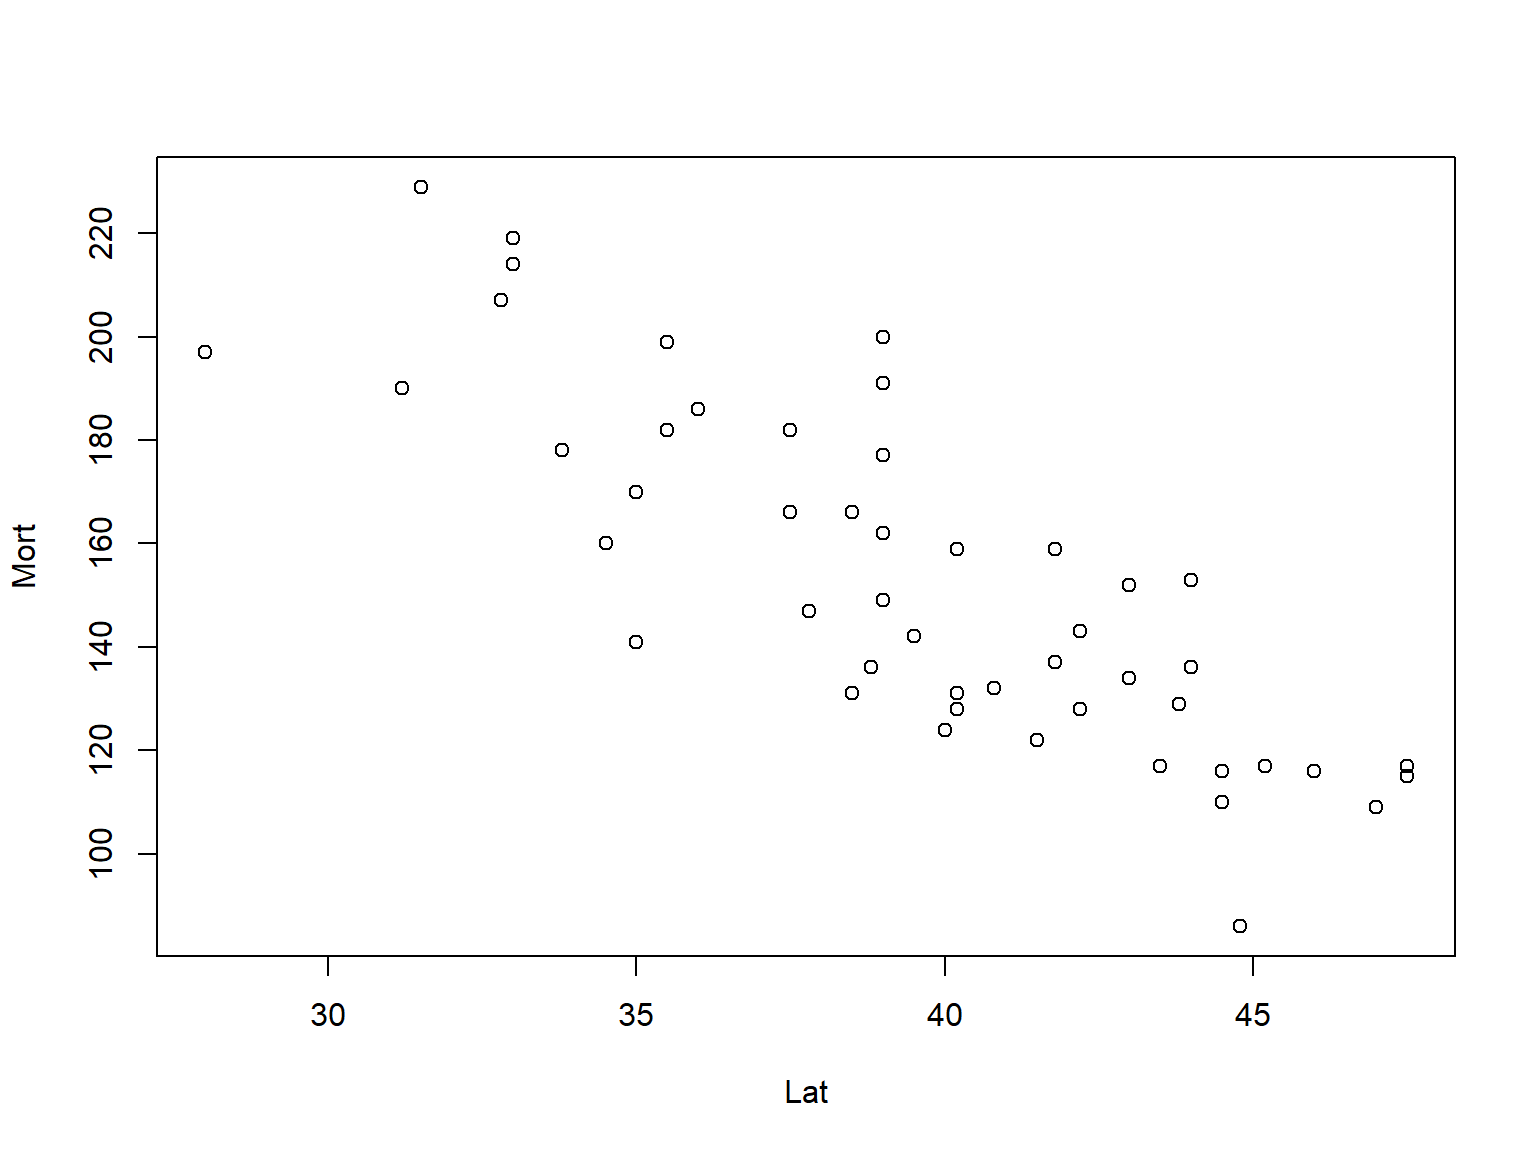
\includegraphics[width=0.5\linewidth]{SMLR_files/figure-latex/unnamed-chunk-28-1} \end{flushleft}

In our R introduction, we used \texttt{ggplot2} to create a more interesting plot. You may also polish a plot with basic functions. Notice it is \emph{huge} in the resulting document, since we have modified some \emph{chunk options} (\texttt{fig.height\ =\ 6,\ fig.width\ =\ 8}) in the RMarkdown file to manipulate its size.

\begin{Shaded}
\begin{Highlighting}[]
  \KeywordTok{plot}\NormalTok{(Mort }\OperatorTok{~}\StringTok{ }\NormalTok{Lat, }\DataTypeTok{data =}\NormalTok{ example_data,}
       \DataTypeTok{xlab =} \StringTok{"Latitude"}\NormalTok{,}
       \DataTypeTok{ylab =} \StringTok{"Skin Cancer Mortality Rate"}\NormalTok{,}
       \DataTypeTok{main =} \StringTok{"Skin Cancer Mortality vs. State Latitude"}\NormalTok{,}
       \DataTypeTok{pch  =} \DecValTok{19}\NormalTok{,}
       \DataTypeTok{cex  =} \FloatTok{1.5}\NormalTok{,}
       \DataTypeTok{col  =} \StringTok{"deepskyblue"}\NormalTok{)}
\end{Highlighting}
\end{Shaded}

\begin{flushleft}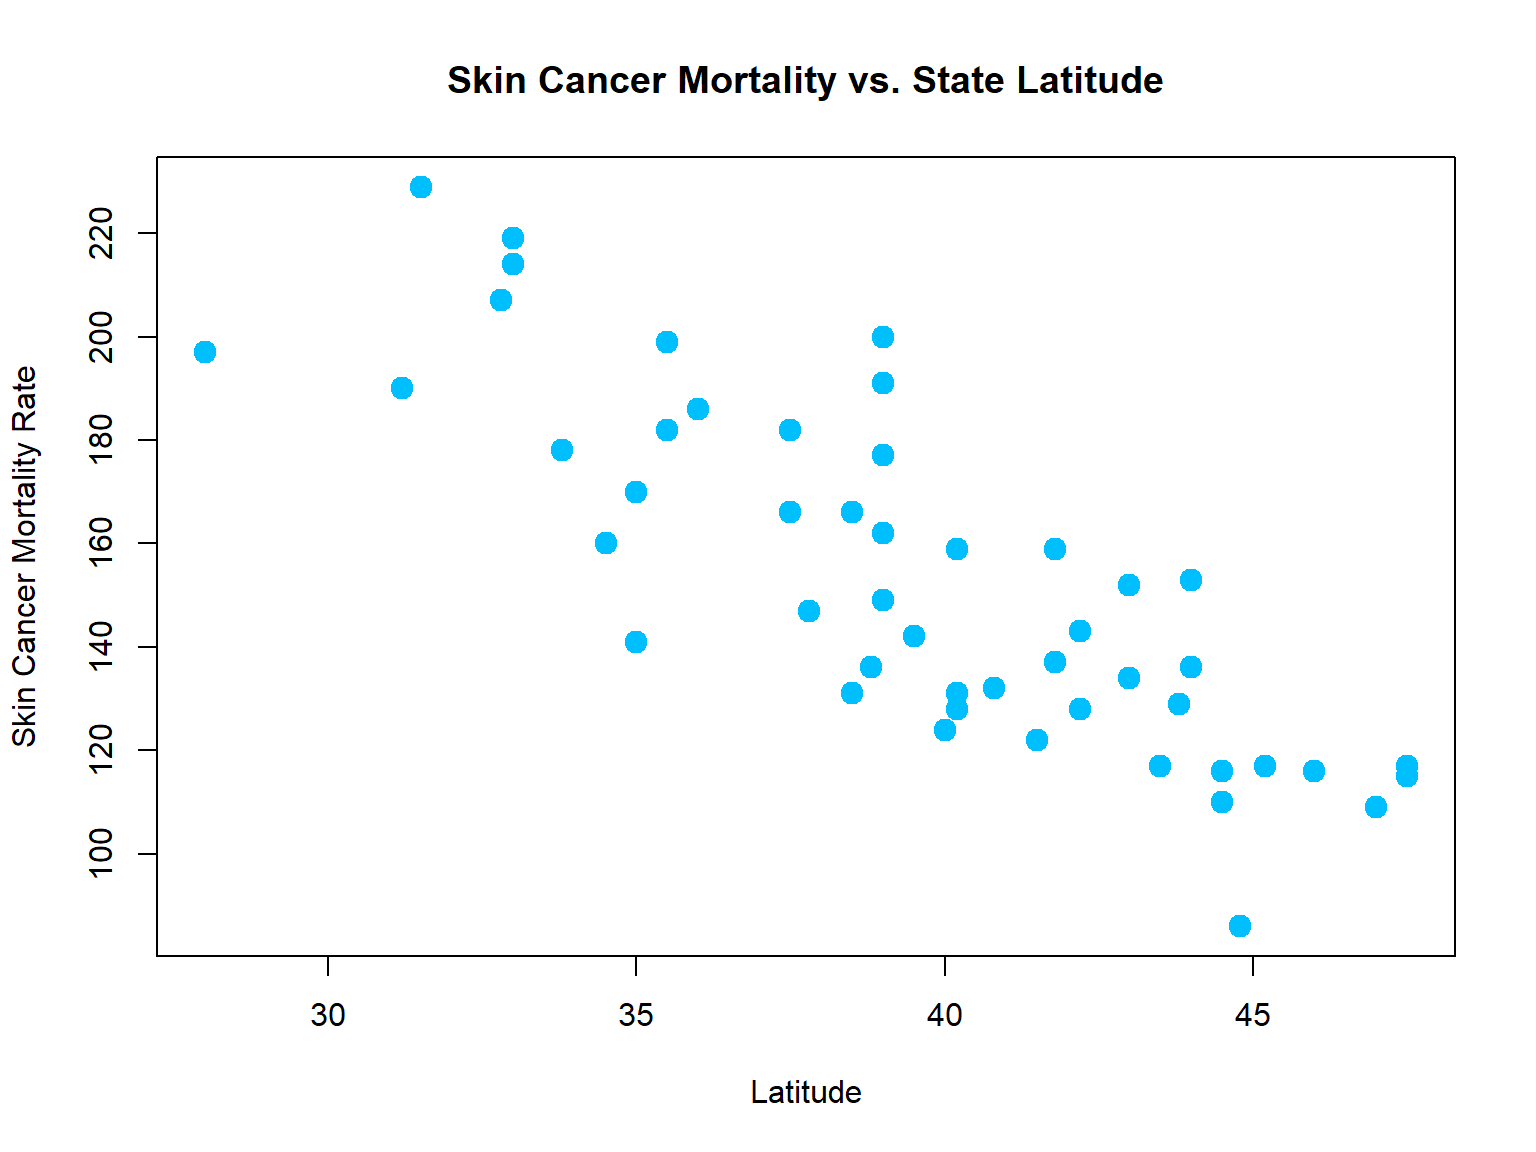
\includegraphics[width=0.5\linewidth]{SMLR_files/figure-latex/unnamed-chunk-29-1} \end{flushleft}

But you can also notice that the labels and the plots becomes disproportional when the figure size is set too small. This can be resolved using a scaling option such as \texttt{out.width\ =\ \textquotesingle{}60\%}, but enlarge the original figure size. We also align the figure at the center using \texttt{fig.align\ =\ \textquotesingle{}center\textquotesingle{}}

\begin{center}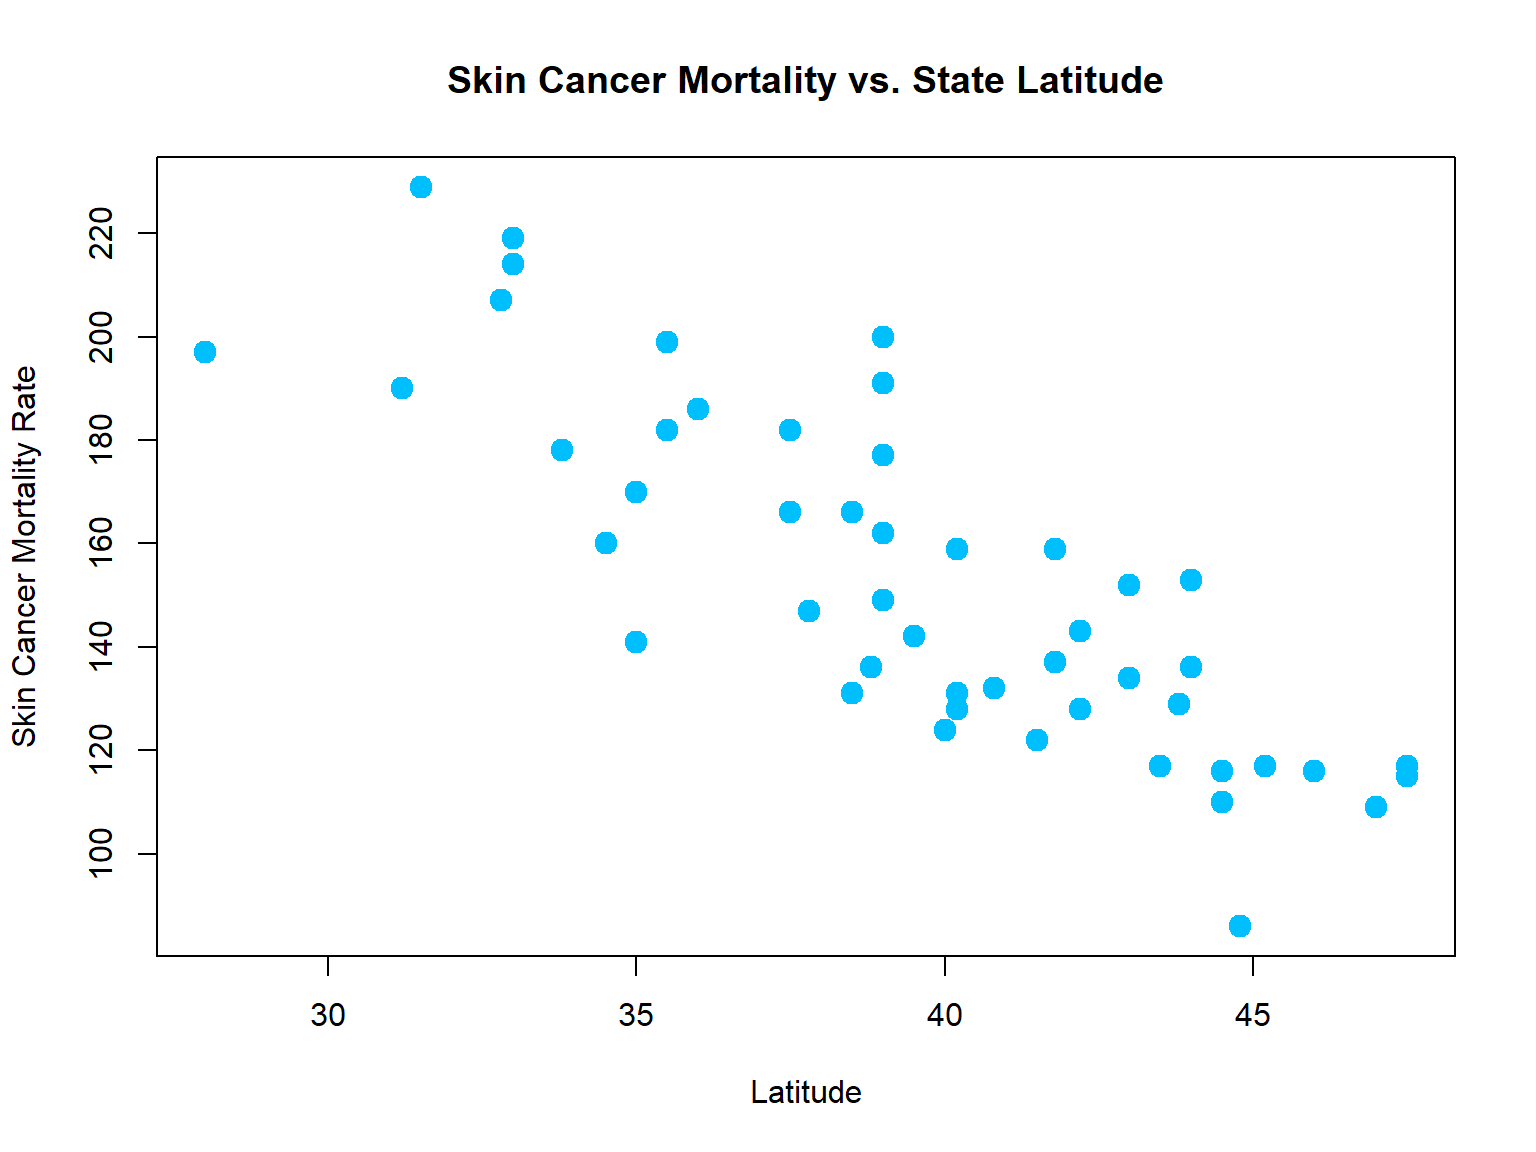
\includegraphics[width=0.6\linewidth]{SMLR_files/figure-latex/unnamed-chunk-30-1} \end{center}

\hypertarget{chunk-options}{%
\section{Chunk Options}\label{chunk-options}}

We have already seen chunk options \texttt{fig.height}, \texttt{fig.width}, and \texttt{out.width} which modified the size of plots from a particular chunk. There are many \href{http://yihui.name/knitr/options/}{chunk options}, but we will discuss some others which are frequently used including; \texttt{eval}, \texttt{echo}, \texttt{message}, and \texttt{warning}. If you noticed, the plot above was displayed without showing the code.

\begin{Shaded}
\begin{Highlighting}[]
  \KeywordTok{install.packages}\NormalTok{(}\StringTok{"rmarkdown"}\NormalTok{)}
\NormalTok{  ?log}
  \KeywordTok{View}\NormalTok{(mpg)}
\end{Highlighting}
\end{Shaded}

Using \texttt{eval\ =\ FALSE} the above chunk displays the code, but it is not run. We've already discussed not wanting install code to run. The \texttt{?} code pulls up documentation of a function. This will spawn a browser window when knitting, or potentially crash during knitting. Similarly, using \texttt{View()} is an issue with RMarkdown. Inside RStudio, this would pull up a window which displays the data. However, when knitting, \texttt{R} runs in the background and RStudio is not modifying the \texttt{View()} function. This, on OSX especially, usually causes knitting to fail.

\begin{verbatim}
## [1] "Hello World!"
\end{verbatim}

Above, we see output, but no code! This is done using \texttt{echo\ =\ FALSE}, which is often useful.

\begin{Shaded}
\begin{Highlighting}[]
\NormalTok{  x =}\StringTok{ }\DecValTok{1}\OperatorTok{:}\DecValTok{10}
\NormalTok{  y =}\StringTok{ }\DecValTok{1}\OperatorTok{:}\DecValTok{10}
  \KeywordTok{summary}\NormalTok{(}\KeywordTok{lm}\NormalTok{(y }\OperatorTok{~}\StringTok{ }\NormalTok{x))}
\end{Highlighting}
\end{Shaded}

\begin{verbatim}
## 
## Call:
## lm(formula = y ~ x)
## 
## Residuals:
##        Min         1Q     Median         3Q        Max 
## -5.661e-16 -1.157e-16  4.273e-17  2.153e-16  4.167e-16 
## 
## Coefficients:
##              Estimate Std. Error   t value Pr(>|t|)    
## (Intercept) 1.123e-15  2.458e-16 4.571e+00  0.00182 ** 
## x           1.000e+00  3.961e-17 2.525e+16  < 2e-16 ***
## ---
## Signif. codes:  0 '***' 0.001 '**' 0.01 '*' 0.05 '.' 0.1 ' ' 1
## 
## Residual standard error: 3.598e-16 on 8 degrees of freedom
## Multiple R-squared:      1,  Adjusted R-squared:      1 
## F-statistic: 6.374e+32 on 1 and 8 DF,  p-value: < 2.2e-16
\end{verbatim}

The above code produces a warning, for reasons we will discuss later. Sometimes, in final reports, it is nice to hide these, which we have done here. \texttt{message\ =\ FALSE} and \texttt{warning\ =\ FALSE} can be used to do so. Messages are often created when loading packages to give the user information about the effects of loading the package. These should be suppressed in final reports. Be careful about suppressing these messages and warnings too early in an analysis as you could potentially miss important information!

\hypertarget{adding-math-with-latex}{%
\section{Adding Math with LaTeX}\label{adding-math-with-latex}}

Another benefit of RMarkdown is the ability to add \href{https://www.latex-project.org/about/}{Latex for mathematics typesetting}. Like \texttt{R} code, there are two ways we can include Latex; displaystyle and inline.

Note that use of LaTeX is somewhat dependent on the resulting file format. For example, it cannot be used at all with \texttt{.docx}. To use it with \texttt{.pdf} you must have LaTeX installed on your machine.

With \texttt{.html} the LaTeX is not actually rendered during knitting, but actually rendered in your browser using MathJax.

\hypertarget{displaystyle-latex}{%
\subsection{Displaystyle LaTeX}\label{displaystyle-latex}}

Displaystyle is used for larger equations which appear centered on their own line. This is done by putting \texttt{\$\$} before and after the mathematical equation.

\[
\widehat \sigma = \sqrt{\frac{1}{n - 1}\sum_{i=1}^{n}(x_i - \bar{x})^2}
\]

\hypertarget{inline-latex}{%
\subsection{Inline LaTex}\label{inline-latex}}

We could mix LaTeX commands in the middle of exposition, for example: \(t = 2\). We could actually mix \texttt{R} with Latex as well! For example: \(\bar{x} = 4.7364838\).

\hypertarget{output-options}{%
\section{Output Options}\label{output-options}}

At the beginning of the document, there is a code which describes some metadata and settings of the document. The default code looks like

\begin{Shaded}
\begin{Highlighting}[]
\NormalTok{  title}\OperatorTok{:}\StringTok{ "R Notebook"}
\NormalTok{  output}\OperatorTok{:}\StringTok{ }\NormalTok{html_notebook}
\end{Highlighting}
\end{Shaded}

You can easily add your name and date to it, and add a Table of Contents, using \texttt{toc:\ yes}. Note that the following code would specify the theme of an \texttt{html} file.

\begin{Shaded}
\begin{Highlighting}[]
\NormalTok{  title}\OperatorTok{:}\StringTok{ "My RMarkdown Template"}
\NormalTok{  author}\OperatorTok{:}\StringTok{ "Your Name"}
\NormalTok{  date}\OperatorTok{:}\StringTok{ "Aug 26, 2021"}
\NormalTok{  output}\OperatorTok{:}
\StringTok{    }\NormalTok{html_document}\OperatorTok{:}\StringTok{ }
\StringTok{      }\NormalTok{toc}\OperatorTok{:}\StringTok{ }\NormalTok{yes}
\end{Highlighting}
\end{Shaded}

You can edit this yourself, or click the settings button at the top of the document and select \texttt{Output\ Options...}. Here you can explore other themes and syntax highlighting options, as well as many additional options. Using this method will automatically modify this information in the document.

\hypertarget{try-it}{%
\section{Try It!}\label{try-it}}

Be sure to play with this document! Change it. Break it. Fix it. The best way to learn RMarkdown (or really almost anything) is to try, fail, then find out what you did wrong.

RStudio has provided a number of \href{http://rmarkdown.rstudio.com/lesson-1.html}{beginner tutorials} which have been greatly improved recently and detail many of the specifics potentially not covered in this document. RMarkdown is continually improving, and this document covers only the very basics.

\hypertarget{linear-regression}{%
\chapter{Linear Regression}\label{linear-regression}}

This chapter severs several purposes. First, we will review some basic knowledge of linear regression. This includes the concept of vector space, projection, which leads to estimating parameters of a linear regression. Most of these knowledge are covered in the prerequisite so you shouldn't find these concepts too difficult to understand. Secondly, we will mainly use the \texttt{lm()} function as an example to demonstrate some features of \texttt{R}. This includes extracting results, visualizations, handling categorical variables, prediction and model selection. These concepts will be useful for other models.

\hypertarget{example-real-estate-data}{%
\section{Example: real estate data}\label{example-real-estate-data}}

This \href{https://archive.ics.uci.edu/ml/datasets/Real+estate+valuation+data+set}{Real Estate data} is provided on the \href{https://archive.ics.uci.edu/ml/index.php}{UCI machine learning repository}. The goal of this dataset is to predict the unit house price based on six different covariates:

\begin{itemize}
\tightlist
\item
  \texttt{date}: The transaction date (for example, 2013.250=2013 March, 2013.500=2013 June, etc.)
\item
  \texttt{age}: The house age (unit: year)
\item
  \texttt{distance}: The distance to the nearest MRT station (unit: meter)
\item
  \texttt{stores}: The number of convenience stores in the living circle on foot (integer)
\item
  \texttt{latitude}: Latitude (unit: degree)
\item
  \texttt{longitude}: Longitude (unit: degree)
\item
  \texttt{price}: House price of unit area
\end{itemize}

\begin{Shaded}
\begin{Highlighting}[]
\NormalTok{    realestate =}\StringTok{ }\KeywordTok{read.csv}\NormalTok{(}\StringTok{"data/realestate.csv"}\NormalTok{, }\DataTypeTok{row.names =} \DecValTok{1}\NormalTok{)}

    \KeywordTok{library}\NormalTok{(DT)}
    \KeywordTok{datatable}\NormalTok{(realestate, }\DataTypeTok{filter =} \StringTok{"top"}\NormalTok{, }\DataTypeTok{rownames =} \OtherTok{FALSE}\NormalTok{,}
              \DataTypeTok{options =} \KeywordTok{list}\NormalTok{(}\DataTypeTok{pageLength =} \DecValTok{8}\NormalTok{))}
\end{Highlighting}
\end{Shaded}

\hypertarget{notation-and-basic-concepts}{%
\section{Notation and Basic Concepts}\label{notation-and-basic-concepts}}

We usually denote the observed covariates data as the design matrix \(\bX\)

Suppose we collect a set of observations with design matrix \(\mathbf{X}\) and outcome \(\mathbf{y}\), linear regression estimate the coefficients through

\[ \widehat{\boldsymbol \beta} = \underset{\boldsymbol \beta}{\arg\min} \big( \mathbf y - \mathbf{X} \boldsymbol \beta \big)^\text{T} \big( \mathbf y - \mathbf{X} \boldsymbol \beta \big) \]
This can be viewed as either a convex optimization problem or projections on the \(n\) dimensional vector space.

\hypertarget{linear-regression-as-an-optimization}{%
\subsection{Linear regression as an optimization}\label{linear-regression-as-an-optimization}}

\begin{Shaded}
\begin{Highlighting}[]
    \CommentTok{# generate data for a simple linear regression }
    \KeywordTok{set.seed}\NormalTok{(}\DecValTok{20}\NormalTok{)}
\NormalTok{    n =}\StringTok{ }\DecValTok{100}
\NormalTok{    x <-}\StringTok{ }\KeywordTok{cbind}\NormalTok{(}\DecValTok{1}\NormalTok{, }\KeywordTok{rnorm}\NormalTok{(n))}
\NormalTok{    y <-}\StringTok{ }\NormalTok{x }\OperatorTok\StringTok{ }\KeywordTok{c}\NormalTok{(}\DecValTok{1}\NormalTok{, }\FloatTok{0.5}\NormalTok{) }\OperatorTok{+}\StringTok{ }\KeywordTok{rnorm}\NormalTok{(n)}
    
    \CommentTok{# calculate the residual sum of squares for a grid of beta values}
\NormalTok{    rss <-}\StringTok{ }\ControlFlowTok{function}\NormalTok{(b, x, y) }\KeywordTok{sum}\NormalTok{((y }\OperatorTok{-}\StringTok{ }\NormalTok{x }\OperatorTok\StringTok{ }\NormalTok{b)}\OperatorTok{^}\DecValTok{2}\NormalTok{)}
\NormalTok{    b1 <-}\StringTok{ }\NormalTok{b2 <-}\StringTok{ }\KeywordTok{seq}\NormalTok{(}\DecValTok{0}\NormalTok{, }\DecValTok{2}\NormalTok{, }\DataTypeTok{length=} \DecValTok{20}\NormalTok{)}
\NormalTok{    z =}\StringTok{ }\KeywordTok{matrix}\NormalTok{(}\KeywordTok{apply}\NormalTok{(}\KeywordTok{expand.grid}\NormalTok{(b1, b2), }\DecValTok{1}\NormalTok{, rss, x, y), }\DecValTok{20}\NormalTok{, }\DecValTok{20}\NormalTok{)}
    
    \CommentTok{# 3d plot for RSS}
    \KeywordTok{par}\NormalTok{(}\DataTypeTok{mar =} \KeywordTok{c}\NormalTok{(}\DecValTok{1}\NormalTok{,}\DecValTok{1}\NormalTok{,}\DecValTok{3}\NormalTok{,}\DecValTok{1}\NormalTok{))}
    \KeywordTok{persp}\NormalTok{(b1, b2, z, }\DataTypeTok{xlab =} \StringTok{"beta 1"}\NormalTok{, }\DataTypeTok{ylab =} \StringTok{"beta 2"}\NormalTok{, }\DataTypeTok{zlab =} \StringTok{"RSS"}\NormalTok{,}
          \DataTypeTok{main=}\StringTok{"Residual Sum of Squares"}\NormalTok{, }\DataTypeTok{col =} \StringTok{"springgreen"}\NormalTok{, }\DataTypeTok{shade =} \FloatTok{0.6}\NormalTok{,}
          \DataTypeTok{theta =} \DecValTok{30}\NormalTok{, }\DataTypeTok{phi =} \DecValTok{5}\NormalTok{)}
\end{Highlighting}
\end{Shaded}

\begin{center}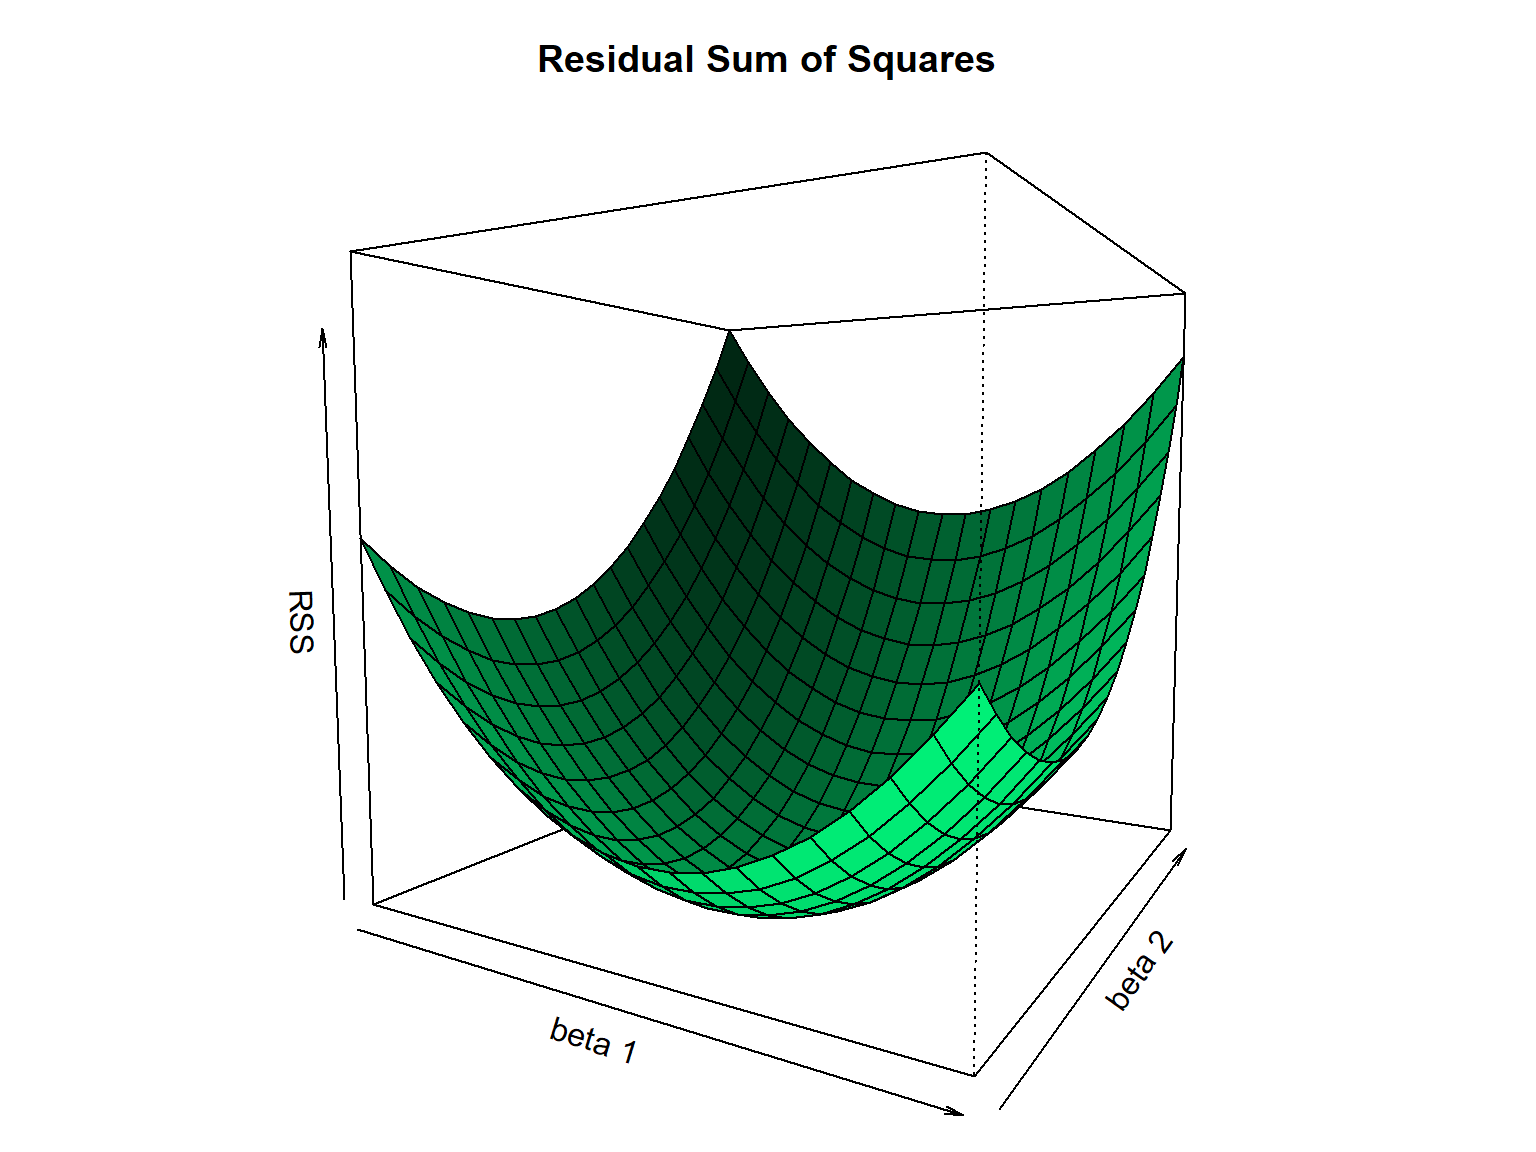
\includegraphics[width=0.6\linewidth]{SMLR_files/figure-latex/unnamed-chunk-37-1} \end{center}

\begin{Shaded}
\begin{Highlighting}[]
    \CommentTok{# The solution can be solved by any optimization algorithm }
    \KeywordTok{optim}\NormalTok{(}\KeywordTok{c}\NormalTok{(}\DecValTok{0}\NormalTok{, }\DecValTok{0}\NormalTok{), rss, }\DataTypeTok{x =}\NormalTok{ x, }\DataTypeTok{y =}\NormalTok{ y)}\OperatorTok{$}\NormalTok{par}
\end{Highlighting}
\end{Shaded}

\begin{verbatim}
## [1] 1.088813 0.679870
\end{verbatim}

\hypertarget{linear-reg}{%
\subsection{Linear regression as projections}\label{linear-reg}}

Another view is through projections in vector space. Consider each column of \(\mathbf{X}\) as a vector, and project \(\mathbf{y}\) onto the column space of \(\mathbf{X}\). The project is

\[ \widehat{\mathbf{y}} = \mathbf{X} (\mathbf{X}^\text{T} \mathbf{X})^{-1}\mathbf{X}^\text{T} \mathbf{y} \doteq {\mathbf{H}} \mathbf{y}, \]
where \(\mathbf{H}\) is a projection matrix. And the residuals are simply

\[ \widehat{\mathbf{e}} = \mathbf{y} - \widehat{\mathbf{y}} = (\mathbf{I} - \mathbf{H}) \mathbf{y} \]
When the number of variables is large, inverting \(\mathbf{X}^\text{T} \mathbf{X}\) is expansive. The \texttt{R} function \texttt{lm()} does not calculate the inverse directly. Instead, QR decomposition can be used. You can try a larger \(n\) and \(p\) to see a significant difference. This is only for demonstration. They are not required for our course.

\begin{Shaded}
\begin{Highlighting}[]
    \CommentTok{# generate 100 observations with 3 variables}
    \KeywordTok{set.seed}\NormalTok{(}\DecValTok{1}\NormalTok{)}
\NormalTok{    n =}\StringTok{ }\DecValTok{1000}
\NormalTok{    p =}\StringTok{ }\DecValTok{500}
\NormalTok{    x =}\StringTok{ }\KeywordTok{matrix}\NormalTok{(}\KeywordTok{rnorm}\NormalTok{(n}\OperatorTok{*}\NormalTok{p), n, p)}
\NormalTok{    X =}\StringTok{ }\KeywordTok{cbind}\NormalTok{(}\DecValTok{1}\NormalTok{, x) }\CommentTok{# the design matrix, including 1 as the first column}
    
    \CommentTok{# define the true beta, the first entry is the intercept}
\NormalTok{    b =}\StringTok{ }\KeywordTok{as.matrix}\NormalTok{(}\KeywordTok{c}\NormalTok{(}\DecValTok{1}\NormalTok{, }\DecValTok{1}\NormalTok{, }\FloatTok{0.5}\NormalTok{, }\KeywordTok{rep}\NormalTok{(}\DecValTok{0}\NormalTok{, p}\DecValTok{-2}\NormalTok{))) }
    
    \CommentTok{# generate training y with Gaussian errors}
\NormalTok{    y =}\StringTok{ }\NormalTok{X }\OperatorTok\StringTok{ }\NormalTok{b }\OperatorTok{+}\StringTok{ }\KeywordTok{rnorm}\NormalTok{(n)}
    
    \CommentTok{# fit a linear regression model }
\NormalTok{    lm.fit =}\StringTok{ }\KeywordTok{lm}\NormalTok{(y }\OperatorTok{~}\StringTok{ }\NormalTok{x)}
    
    \CommentTok{# look at the coefficients beta hat}
    \KeywordTok{head}\NormalTok{(lm.fit}\OperatorTok{$}\NormalTok{coef)}
\end{Highlighting}
\end{Shaded}

\begin{verbatim}
##  (Intercept)           x1           x2           x3           x4           x5 
##  1.016479750  1.026143517  0.496792668 -0.017272409  0.005193304  0.034639107
\end{verbatim}

\begin{Shaded}
\begin{Highlighting}[]
    \CommentTok{# using normal equations by inverting the X'X matrix: b = (X'X)^-1 X'y }
    \CommentTok{# however, this is very slow}
    \CommentTok{# check ?solve}
    \KeywordTok{system.time}\NormalTok{(\{beta_hat =}\StringTok{ }\KeywordTok{solve}\NormalTok{(}\KeywordTok{t}\NormalTok{(X) }\OperatorTok\StringTok{ }\NormalTok{X) }\OperatorTok\StringTok{ }\KeywordTok{t}\NormalTok{(X) }\OperatorTok\StringTok{ }\NormalTok{y\})}
\end{Highlighting}
\end{Shaded}

\begin{verbatim}
##    user  system elapsed 
##    0.32    0.00    0.31
\end{verbatim}

\begin{Shaded}
\begin{Highlighting}[]
    \KeywordTok{head}\NormalTok{(beta_hat)}
\end{Highlighting}
\end{Shaded}

\begin{verbatim}
##              [,1]
## [1,]  1.016479750
## [2,]  1.026143517
## [3,]  0.496792668
## [4,] -0.017272409
## [5,]  0.005193304
## [6,]  0.034639107
\end{verbatim}

\begin{Shaded}
\begin{Highlighting}[]
    \CommentTok{# you can avoid the inversion by specifying the linear equation system X'X b = X'y }
    \KeywordTok{system.time}\NormalTok{(\{beta_hat =}\StringTok{ }\KeywordTok{solve}\NormalTok{(}\KeywordTok{t}\NormalTok{(X) }\OperatorTok\StringTok{ }\NormalTok{X, }\KeywordTok{t}\NormalTok{(X) }\OperatorTok\StringTok{ }\NormalTok{y)\})    }
\end{Highlighting}
\end{Shaded}

\begin{verbatim}
##    user  system elapsed 
##    0.14    0.00    0.14
\end{verbatim}

\begin{Shaded}
\begin{Highlighting}[]
    \CommentTok{# A better approach is to use QR decomposition or the Cholesky decomposition }
    \CommentTok{# The following codes are not necessarily efficient, they are only for demonstration purpose}
    
    \CommentTok{# QR decomposition}
    \CommentTok{# direct calling the qr.coef function}
    \KeywordTok{system.time}\NormalTok{(\{beta_hat =}\StringTok{ }\KeywordTok{qr.coef}\NormalTok{(}\KeywordTok{qr}\NormalTok{(X), y)\})}
\end{Highlighting}
\end{Shaded}

\begin{verbatim}
##    user  system elapsed 
##    0.13    0.02    0.14
\end{verbatim}

\begin{Shaded}
\begin{Highlighting}[]
    \CommentTok{# or }
    \KeywordTok{system.time}\NormalTok{(\{beta_hat =}\StringTok{ }\KeywordTok{qr.solve}\NormalTok{(}\KeywordTok{t}\NormalTok{(X) }\OperatorTok\StringTok{ }\NormalTok{X, }\KeywordTok{t}\NormalTok{(X) }\OperatorTok\StringTok{ }\NormalTok{y)\})}
\end{Highlighting}
\end{Shaded}

\begin{verbatim}
##    user  system elapsed 
##    0.17    0.00    0.17
\end{verbatim}

\begin{Shaded}
\begin{Highlighting}[]
    \CommentTok{# if you want to see what Q and R are}
\NormalTok{    QR =}\StringTok{ }\KeywordTok{qr}\NormalTok{(X)}
\NormalTok{    Q =}\StringTok{ }\KeywordTok{qr.Q}\NormalTok{(QR)}
\NormalTok{    R =}\StringTok{ }\KeywordTok{qr.R}\NormalTok{(QR)}
    
    \CommentTok{# get inverse of R, you can check R %*% R_inv yourself}
    \CommentTok{# the backsolve/forwardsolve functions can be used to solve AX = b for upper/lower triangular matrix A }
    \CommentTok{# ?backsolve}
\NormalTok{    R_inv =}\StringTok{ }\KeywordTok{backsolve}\NormalTok{(R, }\KeywordTok{diag}\NormalTok{(p}\OperatorTok{+}\DecValTok{1}\NormalTok{), }\DataTypeTok{upper.tri =} \OtherTok{TRUE}\NormalTok{, }\DataTypeTok{transpose =} \OtherTok{FALSE}\NormalTok{)}
\NormalTok{    beta_hat =}\StringTok{ }\NormalTok{R_inv }\OperatorTok\StringTok{ }\KeywordTok{t}\NormalTok{(Q) }\OperatorTok\StringTok{ }\NormalTok{y}
    
    \CommentTok{# Cholesky Decomposition }
    
    \CommentTok{# the chol function gives upper triangular matrix}
    \CommentTok{# crossprod(X) = X'X}
    \KeywordTok{system.time}\NormalTok{(\{}
\NormalTok{    R =}\StringTok{ }\KeywordTok{chol}\NormalTok{(}\KeywordTok{crossprod}\NormalTok{(X))}
\NormalTok{    w =}\StringTok{ }\KeywordTok{backsolve}\NormalTok{(R, }\KeywordTok{t}\NormalTok{(X) }\OperatorTok\StringTok{ }\NormalTok{y, }\DataTypeTok{upper.tri =} \OtherTok{TRUE}\NormalTok{, }\DataTypeTok{transpose =} \OtherTok{TRUE}\NormalTok{)}
\NormalTok{    beta_hat =}\StringTok{ }\KeywordTok{backsolve}\NormalTok{(R, w, }\DataTypeTok{upper.tri =} \OtherTok{TRUE}\NormalTok{, }\DataTypeTok{transpose =} \OtherTok{FALSE}\NormalTok{)}
\NormalTok{    \})}
\end{Highlighting}
\end{Shaded}

\begin{verbatim}
##    user  system elapsed 
##    0.13    0.00    0.12
\end{verbatim}

\begin{Shaded}
\begin{Highlighting}[]
    \CommentTok{# or equivalently }
\NormalTok{    R =}\StringTok{ }\KeywordTok{t}\NormalTok{(}\KeywordTok{chol}\NormalTok{(}\KeywordTok{crossprod}\NormalTok{(X)))}
\NormalTok{    w =}\StringTok{ }\KeywordTok{forwardsolve}\NormalTok{(R, }\KeywordTok{t}\NormalTok{(X) }\OperatorTok\StringTok{ }\NormalTok{y, }\DataTypeTok{upper.tri =} \OtherTok{FALSE}\NormalTok{, }\DataTypeTok{transpose =} \OtherTok{FALSE}\NormalTok{)}
\NormalTok{    beta_hat =}\StringTok{ }\KeywordTok{forwardsolve}\NormalTok{(R, w, }\DataTypeTok{upper.tri =} \OtherTok{FALSE}\NormalTok{, }\DataTypeTok{transpose =} \OtherTok{TRUE}\NormalTok{) }\CommentTok{# the transpose = TRUE means that we are solving for R'b = w instead of Rb = w }
\end{Highlighting}
\end{Shaded}

\hypertarget{model-selection-criteria-and-algorithm}{%
\section{Model Selection Criteria and Algorithm}\label{model-selection-criteria-and-algorithm}}

\hypertarget{example-diabetes-dataset}{%
\subsection{\texorpdfstring{Example: \texttt{diabetes} dataset}{Example: diabetes dataset}}\label{example-diabetes-dataset}}

We use the \texttt{diabetes} dataset from the \texttt{lars} package as a demonstration of model selection.

\begin{Shaded}
\begin{Highlighting}[]
    \KeywordTok{library}\NormalTok{(lars)}
    \KeywordTok{data}\NormalTok{(diabetes)}
\NormalTok{    diab =}\StringTok{ }\KeywordTok{data.frame}\NormalTok{(}\KeywordTok{cbind}\NormalTok{(diabetes}\OperatorTok{$}\NormalTok{x, }\StringTok{"Y"}\NormalTok{ =}\StringTok{ }\NormalTok{diabetes}\OperatorTok{$}\NormalTok{y))}
    
    \CommentTok{# A Brief Description of the Diabetes Data (Efron et al, 2004):}
    \CommentTok{# Ten baseline variables: age, sex, body mass index, average blood pressure, and six blood serum}
    \CommentTok{# measurements were obtained for each of n = 442 diabetes patients, as well as}
    \CommentTok{# the response of interest, a quantitative measure of disease progression one year after baseline }
    
\NormalTok{    lmfit=}\KeywordTok{lm}\NormalTok{(Y}\OperatorTok{~}\NormalTok{., }\DataTypeTok{data=}\NormalTok{diab)}
    
    \CommentTok{# When we use normal distribution likelihood for the errors, there are 12 parameters}
    \CommentTok{# The function AIC() directly calculates the AIC score from a lm() fitted model }
\NormalTok{    n =}\StringTok{ }\KeywordTok{nrow}\NormalTok{(diab)}
\NormalTok{    p =}\StringTok{ }\DecValTok{11}

    \CommentTok{# ?AIC}
    \KeywordTok{AIC}\NormalTok{(lmfit) }\CommentTok{# a build-in function for calculating AIC using -2log likelihood}
\end{Highlighting}
\end{Shaded}

\begin{verbatim}
## [1] 4795.985
\end{verbatim}

\begin{Shaded}
\begin{Highlighting}[]
\NormalTok{    n}\OperatorTok{*}\KeywordTok{log}\NormalTok{(}\KeywordTok{sum}\NormalTok{(}\KeywordTok{residuals}\NormalTok{(lmfit)}\OperatorTok{^}\DecValTok{2}\OperatorTok{/}\NormalTok{n)) }\OperatorTok{+}\StringTok{ }\NormalTok{n }\OperatorTok{+}\StringTok{ }\NormalTok{n}\OperatorTok{*}\KeywordTok{log}\NormalTok{(}\DecValTok{2}\OperatorTok{*}\NormalTok{pi) }\OperatorTok{+}\StringTok{ }\DecValTok{2} \OperatorTok{+}\StringTok{ }\DecValTok{2}\OperatorTok{*}\NormalTok{p}
\end{Highlighting}
\end{Shaded}

\begin{verbatim}
## [1] 4795.985
\end{verbatim}

\begin{Shaded}
\begin{Highlighting}[]
    \CommentTok{# In many standard R packages, the AIC is calculated by removing some constants from the likelihood }
    \CommentTok{# We will use this value as the default}
    
    \CommentTok{# ?extractAIC}
    \KeywordTok{extractAIC}\NormalTok{(lmfit) }\CommentTok{# AIC for the full model}
\end{Highlighting}
\end{Shaded}

\begin{verbatim}
## [1]   11.000 3539.643
\end{verbatim}

\begin{Shaded}
\begin{Highlighting}[]
\NormalTok{    RSS =}\StringTok{ }\KeywordTok{sum}\NormalTok{(}\KeywordTok{residuals}\NormalTok{(lmfit)}\OperatorTok{^}\DecValTok{2}\NormalTok{)}
\NormalTok{    n}\OperatorTok{*}\KeywordTok{log}\NormalTok{(RSS}\OperatorTok{/}\NormalTok{n) }\OperatorTok{+}\StringTok{ }\DecValTok{2}\OperatorTok{*}\NormalTok{p}
\end{Highlighting}
\end{Shaded}

\begin{verbatim}
## [1] 3539.643
\end{verbatim}

\begin{Shaded}
\begin{Highlighting}[]
    \CommentTok{# so the BIC for the full model is }
    \KeywordTok{extractAIC}\NormalTok{(lmfit, }\DataTypeTok{k =} \KeywordTok{log}\NormalTok{(n))}
\end{Highlighting}
\end{Shaded}

\begin{verbatim}
## [1]   11.000 3584.648
\end{verbatim}

\begin{Shaded}
\begin{Highlighting}[]
\NormalTok{    n}\OperatorTok{*}\KeywordTok{log}\NormalTok{(RSS}\OperatorTok{/}\NormalTok{n) }\OperatorTok{+}\StringTok{ }\KeywordTok{log}\NormalTok{(n)}\OperatorTok{*}\NormalTok{p}
\end{Highlighting}
\end{Shaded}

\begin{verbatim}
## [1] 3584.648
\end{verbatim}

\begin{Shaded}
\begin{Highlighting}[]
    \CommentTok{# if we want to calculate Cp, use the formula}
\NormalTok{    RSS }\OperatorTok{+}\StringTok{ }\DecValTok{2}\OperatorTok{*}\NormalTok{p}\OperatorTok{*}\KeywordTok{summary}\NormalTok{(lmfit)}\OperatorTok{$}\NormalTok{sigma}\OperatorTok{^}\DecValTok{2}
\end{Highlighting}
\end{Shaded}

\begin{verbatim}
## [1] 1328502
\end{verbatim}

\begin{Shaded}
\begin{Highlighting}[]
    \CommentTok{# however, the scale of this is usually very large, we may consider the following version}
\NormalTok{    RSS}\OperatorTok{/}\KeywordTok{summary}\NormalTok{(lmfit)}\OperatorTok{$}\NormalTok{sigma}\OperatorTok{^}\DecValTok{2} \OperatorTok{+}\StringTok{ }\DecValTok{2}\OperatorTok{*}\NormalTok{p }\OperatorTok{-}\StringTok{ }\NormalTok{n}
\end{Highlighting}
\end{Shaded}

\begin{verbatim}
## [1] 11
\end{verbatim}

The \texttt{step()} function can be used to select the best model based on specified model selection criteria.

\begin{Shaded}
\begin{Highlighting}[]
    \CommentTok{# Model selection: stepwise algorithm }
    \CommentTok{# ?step}
    
    \CommentTok{# this function shows every step during the model selection }
    \KeywordTok{step}\NormalTok{(lmfit, }\DataTypeTok{direction=}\StringTok{"both"}\NormalTok{, }\DataTypeTok{k =} \DecValTok{2}\NormalTok{)    }\CommentTok{# k = 2 (AIC) is default; }
\end{Highlighting}
\end{Shaded}

\begin{verbatim}
## Start:  AIC=3539.64
## Y ~ age + sex + bmi + map + tc + ldl + hdl + tch + ltg + glu
## 
##        Df Sum of Sq     RSS    AIC
## - age   1        82 1264066 3537.7
## - hdl   1       663 1264646 3537.9
## - glu   1      3080 1267064 3538.7
## - tch   1      3526 1267509 3538.9
## <none>              1263983 3539.6
## - ldl   1      5799 1269782 3539.7
## - tc    1     10600 1274583 3541.3
## - sex   1     45000 1308983 3553.1
## - ltg   1     56015 1319998 3556.8
## - map   1     72103 1336086 3562.2
## - bmi   1    179028 1443011 3596.2
## 
## Step:  AIC=3537.67
## Y ~ sex + bmi + map + tc + ldl + hdl + tch + ltg + glu
## 
##        Df Sum of Sq     RSS    AIC
## - hdl   1       646 1264712 3535.9
## - glu   1      3001 1267067 3536.7
## - tch   1      3543 1267608 3536.9
## <none>              1264066 3537.7
## - ldl   1      5751 1269817 3537.7
## - tc    1     10569 1274635 3539.4
## + age   1        82 1263983 3539.6
## - sex   1     45831 1309896 3551.4
## - ltg   1     55963 1320029 3554.8
## - map   1     73850 1337915 3560.8
## - bmi   1    179079 1443144 3594.2
## 
## Step:  AIC=3535.9
## Y ~ sex + bmi + map + tc + ldl + tch + ltg + glu
## 
##        Df Sum of Sq     RSS    AIC
## - glu   1      3093 1267805 3535.0
## - tch   1      3247 1267959 3535.0
## <none>              1264712 3535.9
## - ldl   1      7505 1272217 3536.5
## + hdl   1       646 1264066 3537.7
## + age   1        66 1264646 3537.9
## - tc    1     26840 1291552 3543.2
## - sex   1     46382 1311094 3549.8
## - map   1     73536 1338248 3558.9
## - ltg   1     97509 1362221 3566.7
## - bmi   1    178537 1443249 3592.3
## 
## Step:  AIC=3534.98
## Y ~ sex + bmi + map + tc + ldl + tch + ltg
## 
##        Df Sum of Sq     RSS    AIC
## - tch   1      3686 1271491 3534.3
## <none>              1267805 3535.0
## - ldl   1      7472 1275277 3535.6
## + glu   1      3093 1264712 3535.9
## + hdl   1       738 1267067 3536.7
## + age   1         0 1267805 3537.0
## - tc    1     26378 1294183 3542.1
## - sex   1     44686 1312491 3548.3
## - map   1     82154 1349959 3560.7
## - ltg   1    102520 1370325 3567.3
## - bmi   1    189970 1457775 3594.7
## 
## Step:  AIC=3534.26
## Y ~ sex + bmi + map + tc + ldl + ltg
## 
##        Df Sum of Sq     RSS    AIC
## <none>              1271491 3534.3
## + tch   1      3686 1267805 3535.0
## + glu   1      3532 1267959 3535.0
## + hdl   1       395 1271097 3536.1
## + age   1        11 1271480 3536.3
## - ldl   1     39378 1310869 3545.7
## - sex   1     41858 1313349 3546.6
## - tc    1     65237 1336728 3554.4
## - map   1     79627 1351119 3559.1
## - bmi   1    190586 1462077 3594.0
## - ltg   1    294094 1565585 3624.2
\end{verbatim}

\begin{verbatim}
## 
## Call:
## lm(formula = Y ~ sex + bmi + map + tc + ldl + ltg, data = diab)
## 
## Coefficients:
## (Intercept)          sex          bmi          map           tc          ldl          ltg  
##       152.1       -226.5        529.9        327.2       -757.9        538.6        804.2
\end{verbatim}

\begin{Shaded}
\begin{Highlighting}[]
    \KeywordTok{step}\NormalTok{(lmfit, }\DataTypeTok{direction=}\StringTok{"backward"}\NormalTok{, }\DataTypeTok{trace=}\DecValTok{0}\NormalTok{) }\CommentTok{# trace=0 will not print intermediate results}
\end{Highlighting}
\end{Shaded}

\begin{verbatim}
## 
## Call:
## lm(formula = Y ~ sex + bmi + map + tc + ldl + ltg, data = diab)
## 
## Coefficients:
## (Intercept)          sex          bmi          map           tc          ldl          ltg  
##       152.1       -226.5        529.9        327.2       -757.9        538.6        804.2
\end{verbatim}

\begin{Shaded}
\begin{Highlighting}[]
    \KeywordTok{step}\NormalTok{(}\KeywordTok{lm}\NormalTok{(Y}\OperatorTok{~}\DecValTok{1}\NormalTok{, }\DataTypeTok{data=}\NormalTok{diab), }\DataTypeTok{scope=}\KeywordTok{list}\NormalTok{(}\DataTypeTok{upper=}\NormalTok{lmfit, }\DataTypeTok{lower=}\OperatorTok{~}\DecValTok{1}\NormalTok{), }\DataTypeTok{direction=}\StringTok{"forward"}\NormalTok{, }\DataTypeTok{trace=}\DecValTok{0}\NormalTok{)}
\end{Highlighting}
\end{Shaded}

\begin{verbatim}
## 
## Call:
## lm(formula = Y ~ bmi + ltg + map + tc + sex + ldl, data = diab)
## 
## Coefficients:
## (Intercept)          bmi          ltg          map           tc          sex          ldl  
##       152.1        529.9        804.2        327.2       -757.9       -226.5        538.6
\end{verbatim}

\begin{Shaded}
\begin{Highlighting}[]
    \KeywordTok{step}\NormalTok{(lmfit, }\DataTypeTok{direction=}\StringTok{"both"}\NormalTok{, }\DataTypeTok{k=}\KeywordTok{log}\NormalTok{(n), }\DataTypeTok{trace=}\DecValTok{0}\NormalTok{)  }\CommentTok{# BIC (the default value for k=2, which corresponds to AIC)}
\end{Highlighting}
\end{Shaded}

\begin{verbatim}
## 
## Call:
## lm(formula = Y ~ sex + bmi + map + tc + ldl + ltg, data = diab)
## 
## Coefficients:
## (Intercept)          sex          bmi          map           tc          ldl          ltg  
##       152.1       -226.5        529.9        327.2       -757.9        538.6        804.2
\end{verbatim}

The \texttt{leaps} package will calculate the best model of each model size. Then we can add the penalties to the model fitting result and conclude the best model.

\begin{Shaded}
\begin{Highlighting}[]
    \CommentTok{##########################################################################}
    \CommentTok{# Best subset model selection (Cp, AIC, and BIC): leaps }
    \CommentTok{##########################################################################}
    \KeywordTok{library}\NormalTok{(leaps)}
    
    \CommentTok{# performs an exhaustive search over models, and gives back the best model }
    \CommentTok{# (with low RSS) of each size.}
    \CommentTok{# the default maximum model size is nvmax=8}
    
\NormalTok{    RSSleaps=}\KeywordTok{regsubsets}\NormalTok{(}\KeywordTok{as.matrix}\NormalTok{(diab[,}\OperatorTok{-}\DecValTok{11}\NormalTok{]),diab[,}\DecValTok{11}\NormalTok{])}
    \KeywordTok{summary}\NormalTok{(RSSleaps, }\DataTypeTok{matrix=}\NormalTok{T)}
\end{Highlighting}
\end{Shaded}

\begin{verbatim}
## Subset selection object
## 10 Variables  (and intercept)
##     Forced in Forced out
## age     FALSE      FALSE
## sex     FALSE      FALSE
## bmi     FALSE      FALSE
## map     FALSE      FALSE
## tc      FALSE      FALSE
## ldl     FALSE      FALSE
## hdl     FALSE      FALSE
## tch     FALSE      FALSE
## ltg     FALSE      FALSE
## glu     FALSE      FALSE
## 1 subsets of each size up to 8
## Selection Algorithm: exhaustive
##          age sex bmi map tc  ldl hdl tch ltg glu
## 1  ( 1 ) " " " " "*" " " " " " " " " " " " " " "
## 2  ( 1 ) " " " " "*" " " " " " " " " " " "*" " "
## 3  ( 1 ) " " " " "*" "*" " " " " " " " " "*" " "
## 4  ( 1 ) " " " " "*" "*" "*" " " " " " " "*" " "
## 5  ( 1 ) " " "*" "*" "*" " " " " "*" " " "*" " "
## 6  ( 1 ) " " "*" "*" "*" "*" "*" " " " " "*" " "
## 7  ( 1 ) " " "*" "*" "*" "*" "*" " " "*" "*" " "
## 8  ( 1 ) " " "*" "*" "*" "*" "*" " " "*" "*" "*"
\end{verbatim}

\begin{Shaded}
\begin{Highlighting}[]
\NormalTok{    RSSleaps=}\KeywordTok{regsubsets}\NormalTok{(}\KeywordTok{as.matrix}\NormalTok{(diab[,}\OperatorTok{-}\DecValTok{11}\NormalTok{]),diab[,}\DecValTok{11}\NormalTok{], }\DataTypeTok{nvmax=}\DecValTok{10}\NormalTok{)}
    \KeywordTok{summary}\NormalTok{(RSSleaps,}\DataTypeTok{matrix=}\NormalTok{T)}
\end{Highlighting}
\end{Shaded}

\begin{verbatim}
## Subset selection object
## 10 Variables  (and intercept)
##     Forced in Forced out
## age     FALSE      FALSE
## sex     FALSE      FALSE
## bmi     FALSE      FALSE
## map     FALSE      FALSE
## tc      FALSE      FALSE
## ldl     FALSE      FALSE
## hdl     FALSE      FALSE
## tch     FALSE      FALSE
## ltg     FALSE      FALSE
## glu     FALSE      FALSE
## 1 subsets of each size up to 10
## Selection Algorithm: exhaustive
##           age sex bmi map tc  ldl hdl tch ltg glu
## 1  ( 1 )  " " " " "*" " " " " " " " " " " " " " "
## 2  ( 1 )  " " " " "*" " " " " " " " " " " "*" " "
## 3  ( 1 )  " " " " "*" "*" " " " " " " " " "*" " "
## 4  ( 1 )  " " " " "*" "*" "*" " " " " " " "*" " "
## 5  ( 1 )  " " "*" "*" "*" " " " " "*" " " "*" " "
## 6  ( 1 )  " " "*" "*" "*" "*" "*" " " " " "*" " "
## 7  ( 1 )  " " "*" "*" "*" "*" "*" " " "*" "*" " "
## 8  ( 1 )  " " "*" "*" "*" "*" "*" " " "*" "*" "*"
## 9  ( 1 )  " " "*" "*" "*" "*" "*" "*" "*" "*" "*"
## 10  ( 1 ) "*" "*" "*" "*" "*" "*" "*" "*" "*" "*"
\end{verbatim}

\begin{Shaded}
\begin{Highlighting}[]
\NormalTok{    sumleaps=}\KeywordTok{summary}\NormalTok{(RSSleaps,}\DataTypeTok{matrix=}\NormalTok{T)}
    \KeywordTok{names}\NormalTok{(sumleaps)  }\CommentTok{# components returned by summary(RSSleaps)}
\end{Highlighting}
\end{Shaded}

\begin{verbatim}
## [1] "which"  "rsq"    "rss"    "adjr2"  "cp"     "bic"    "outmat" "obj"
\end{verbatim}

\begin{Shaded}
\begin{Highlighting}[]
\NormalTok{    sumleaps}\OperatorTok{$}\NormalTok{which}
\end{Highlighting}
\end{Shaded}

\begin{verbatim}
##    (Intercept)   age   sex  bmi   map    tc   ldl   hdl   tch   ltg   glu
## 1         TRUE FALSE FALSE TRUE FALSE FALSE FALSE FALSE FALSE FALSE FALSE
## 2         TRUE FALSE FALSE TRUE FALSE FALSE FALSE FALSE FALSE  TRUE FALSE
## 3         TRUE FALSE FALSE TRUE  TRUE FALSE FALSE FALSE FALSE  TRUE FALSE
## 4         TRUE FALSE FALSE TRUE  TRUE  TRUE FALSE FALSE FALSE  TRUE FALSE
## 5         TRUE FALSE  TRUE TRUE  TRUE FALSE FALSE  TRUE FALSE  TRUE FALSE
## 6         TRUE FALSE  TRUE TRUE  TRUE  TRUE  TRUE FALSE FALSE  TRUE FALSE
## 7         TRUE FALSE  TRUE TRUE  TRUE  TRUE  TRUE FALSE  TRUE  TRUE FALSE
## 8         TRUE FALSE  TRUE TRUE  TRUE  TRUE  TRUE FALSE  TRUE  TRUE  TRUE
## 9         TRUE FALSE  TRUE TRUE  TRUE  TRUE  TRUE  TRUE  TRUE  TRUE  TRUE
## 10        TRUE  TRUE  TRUE TRUE  TRUE  TRUE  TRUE  TRUE  TRUE  TRUE  TRUE
\end{verbatim}

\begin{Shaded}
\begin{Highlighting}[]
\NormalTok{    msize=}\KeywordTok{apply}\NormalTok{(sumleaps}\OperatorTok{$}\NormalTok{which,}\DecValTok{1}\NormalTok{,sum)}
\NormalTok{    n=}\KeywordTok{dim}\NormalTok{(diab)[}\DecValTok{1}\NormalTok{]}
\NormalTok{    p=}\KeywordTok{dim}\NormalTok{(diab)[}\DecValTok{2}\NormalTok{]}
\NormalTok{    Cp =}\StringTok{ }\NormalTok{sumleaps}\OperatorTok{$}\NormalTok{rss}\OperatorTok{/}\NormalTok{(}\KeywordTok{summary}\NormalTok{(lmfit)}\OperatorTok{$}\NormalTok{sigma}\OperatorTok{^}\DecValTok{2}\NormalTok{) }\OperatorTok{+}\StringTok{ }\DecValTok{2}\OperatorTok{*}\NormalTok{msize }\OperatorTok{-}\StringTok{ }\NormalTok{n;}
\NormalTok{    AIC =}\StringTok{ }\NormalTok{n}\OperatorTok{*}\KeywordTok{log}\NormalTok{(sumleaps}\OperatorTok{$}\NormalTok{rss}\OperatorTok{/}\NormalTok{n) }\OperatorTok{+}\StringTok{ }\DecValTok{2}\OperatorTok{*}\NormalTok{msize;}
\NormalTok{    BIC =}\StringTok{ }\NormalTok{n}\OperatorTok{*}\KeywordTok{log}\NormalTok{(sumleaps}\OperatorTok{$}\NormalTok{rss}\OperatorTok{/}\NormalTok{n) }\OperatorTok{+}\StringTok{ }\NormalTok{msize}\OperatorTok{*}\KeywordTok{log}\NormalTok{(n);}
    
    \KeywordTok{cbind}\NormalTok{(Cp, sumleaps}\OperatorTok{$}\NormalTok{cp)}
\end{Highlighting}
\end{Shaded}

\begin{verbatim}
##            Cp           
## 1  148.352561 148.352561
## 2   47.072229  47.072229
## 3   30.663634  30.663634
## 4   21.998461  21.998461
## 5    9.148045   9.148045
## 6    5.560162   5.560162
## 7    6.303221   6.303221
## 8    7.248522   7.248522
## 9    9.028080   9.028080
## 10  11.000000  11.000000
\end{verbatim}

\begin{Shaded}
\begin{Highlighting}[]
    \KeywordTok{cbind}\NormalTok{(BIC, sumleaps}\OperatorTok{$}\NormalTok{bic)  }\CommentTok{# It seems regsubsets uses a formula for BIC different from the one we used. }
\end{Highlighting}
\end{Shaded}

\begin{verbatim}
##         BIC          
## 1  3665.879 -174.1108
## 2  3586.331 -253.6592
## 3  3575.249 -264.7407
## 4  3571.077 -268.9126
## 5  3562.469 -277.5210
## 6  3562.900 -277.0899
## 7  3567.708 -272.2819
## 8  3572.720 -267.2702
## 9  3578.585 -261.4049
## 10 3584.648 -255.3424
\end{verbatim}

\begin{Shaded}
\begin{Highlighting}[]
\NormalTok{    BIC}\OperatorTok{-}\NormalTok{sumleaps}\OperatorTok{$}\NormalTok{bic  }\CommentTok{# But the two just differ by a constant, so won't affect the model selection result. }
\end{Highlighting}
\end{Shaded}

\begin{verbatim}
##       1       2       3       4       5       6       7       8       9      10 
## 3839.99 3839.99 3839.99 3839.99 3839.99 3839.99 3839.99 3839.99 3839.99 3839.99
\end{verbatim}

\begin{Shaded}
\begin{Highlighting}[]
\NormalTok{    n}\OperatorTok{*}\KeywordTok{log}\NormalTok{(}\KeywordTok{sum}\NormalTok{((diab[,}\DecValTok{11}\NormalTok{] }\OperatorTok{-}\StringTok{ }\KeywordTok{mean}\NormalTok{(diab[,}\DecValTok{11}\NormalTok{]))}\OperatorTok{^}\DecValTok{2}\OperatorTok{/}\NormalTok{n)) }\CommentTok{# the difference is the score of an intercept model}
\end{Highlighting}
\end{Shaded}

\begin{verbatim}
## [1] 3839.99
\end{verbatim}

\begin{Shaded}
\begin{Highlighting}[]
    \CommentTok{# Rescale Cp, AIC, BIC to (0,1).}
\NormalTok{    inrange <-}\StringTok{ }\ControlFlowTok{function}\NormalTok{(x) \{ (x }\OperatorTok{-}\StringTok{ }\KeywordTok{min}\NormalTok{(x)) }\OperatorTok{/}\StringTok{ }\NormalTok{(}\KeywordTok{max}\NormalTok{(x) }\OperatorTok{-}\StringTok{ }\KeywordTok{min}\NormalTok{(x)) \}}
    
\NormalTok{    Cp =}\StringTok{ }\NormalTok{sumleaps}\OperatorTok{$}\NormalTok{cp; Cp =}\StringTok{ }\KeywordTok{inrange}\NormalTok{(Cp);}
\NormalTok{    BIC =}\StringTok{ }\NormalTok{sumleaps}\OperatorTok{$}\NormalTok{bic; BIC =}\StringTok{ }\KeywordTok{inrange}\NormalTok{(BIC);}
\NormalTok{    AIC =}\StringTok{ }\NormalTok{n}\OperatorTok{*}\KeywordTok{log}\NormalTok{(sumleaps}\OperatorTok{$}\NormalTok{rss}\OperatorTok{/}\NormalTok{n) }\OperatorTok{+}\StringTok{ }\DecValTok{2}\OperatorTok{*}\NormalTok{msize; AIC =}\StringTok{ }\KeywordTok{inrange}\NormalTok{(AIC);}
    
    \KeywordTok{plot}\NormalTok{(}\KeywordTok{range}\NormalTok{(msize), }\KeywordTok{c}\NormalTok{(}\DecValTok{0}\NormalTok{, }\FloatTok{1.1}\NormalTok{), }\DataTypeTok{type=}\StringTok{"n"}\NormalTok{, }
         \DataTypeTok{xlab=}\StringTok{"Model Size (with Intercept)"}\NormalTok{, }\DataTypeTok{ylab=}\StringTok{"Model Selection Criteria"}\NormalTok{)}
    \KeywordTok{points}\NormalTok{(msize, Cp, }\DataTypeTok{col=}\StringTok{"red"}\NormalTok{, }\DataTypeTok{type=}\StringTok{"b"}\NormalTok{)}
    \KeywordTok{points}\NormalTok{(msize, AIC, }\DataTypeTok{col=}\StringTok{"blue"}\NormalTok{, }\DataTypeTok{type=}\StringTok{"b"}\NormalTok{)}
    \KeywordTok{points}\NormalTok{(msize, BIC, }\DataTypeTok{col=}\StringTok{"black"}\NormalTok{, }\DataTypeTok{type=}\StringTok{"b"}\NormalTok{)}
    \KeywordTok{legend}\NormalTok{(}\StringTok{"topright"}\NormalTok{, }\DataTypeTok{lty=}\KeywordTok{rep}\NormalTok{(}\DecValTok{1}\NormalTok{,}\DecValTok{3}\NormalTok{), }\DataTypeTok{col=}\KeywordTok{c}\NormalTok{(}\StringTok{"red"}\NormalTok{, }\StringTok{"blue"}\NormalTok{, }\StringTok{"black"}\NormalTok{), }\DataTypeTok{legend=}\KeywordTok{c}\NormalTok{(}\StringTok{"Cp"}\NormalTok{, }\StringTok{"AIC"}\NormalTok{, }\StringTok{"BIC"}\NormalTok{))}
\end{Highlighting}
\end{Shaded}

\begin{center}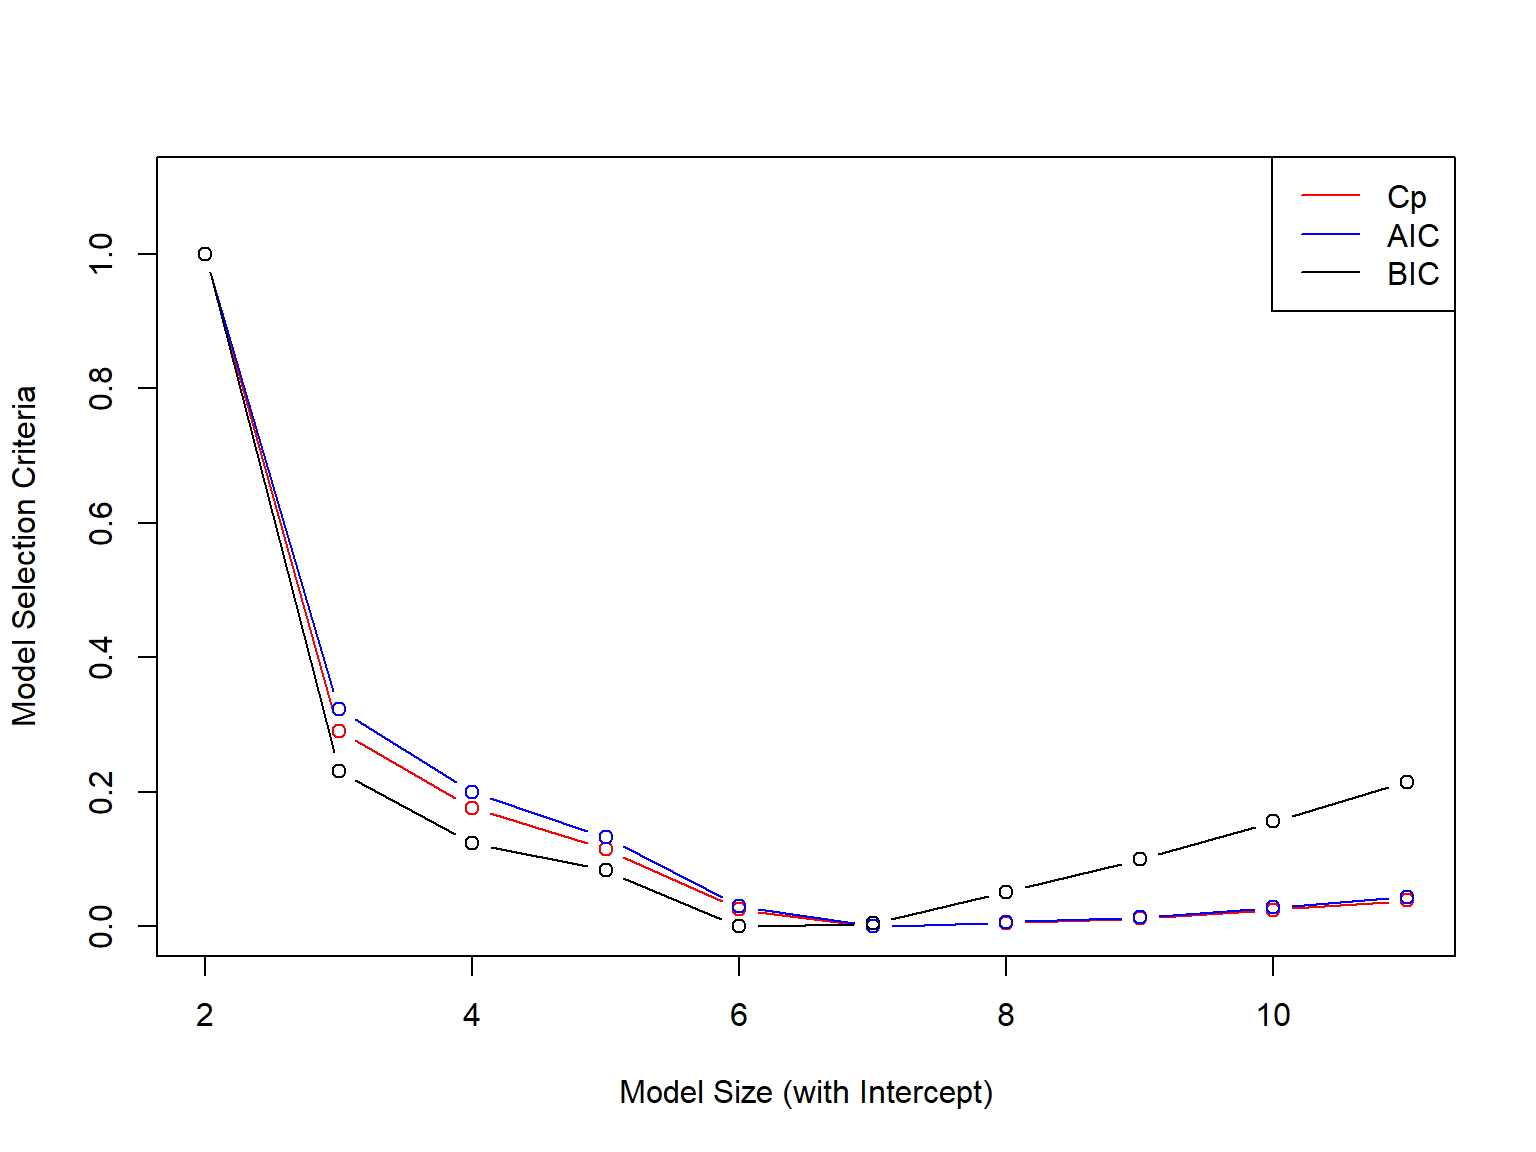
\includegraphics[width=0.6\linewidth]{SMLR_files/figure-latex/unnamed-chunk-41-1} \end{center}

\hypertarget{refs}{}
\leavevmode\hypertarget{ref-hastie2001elements}{}%
Hastie, Trevor, Robert Tibshirani, and Jerome Friedman. 2001. \emph{The Elements of Statistical Learning}. Vol. 1. Springer series in statistics New York.

\leavevmode\hypertarget{ref-james2013introduction}{}%
James, Gareth, Daniela Witten, Trevor Hastie, and Robert Tibshirani. 2013. \emph{An Introduction to Statistical Learning}. Vol. 112. Springer.

\end{document}
